\documentclass[conference]{IEEEtran}[10pt]
\IEEEoverridecommandlockouts

\usepackage{cite}
\usepackage{amsmath,amssymb,amsfonts}
\usepackage{algorithmic}
\usepackage{graphicx}
\usepackage{textcomp}
\usepackage{xcolor}
\def\BibTeX{{\rm B\kern-.05em{\sc i\kern-.025em b}\kern-.08em
    T\kern-.1667em\lower.7ex\hbox{E}\kern-.125emX}}


\usepackage[utf8]{inputenc}
% Auskommentieren sofern Deutsch
\usepackage[ngerman]{babel}
\usepackage{pgfplots}
\usepackage{url}

\usepackage{subcaption}
\usepackage[hidelinks]{hyperref}

\usepackage{pgfplots}
\pgfplotsset{compat=1.17}

\usepackage{tikz}
\usetikzlibrary{positioning,fit,shapes.geometric,backgrounds}

\begin{document}


%\title{Ship Tracking in 2D Using Unscented Kalman Filters: Implementation, Analysis and Evaluation of Effectiveness for Direction, Distance and Angle Estimations}

\title{Lokalisierung in 2D mit Unscented Kalman Filtern: Implementierung, Analyse und Bewertung der Effektivität für Richtungs-, Distanz- und Winkelschätzungen}

\author{\IEEEauthorblockN{M.M., S. M., T.K}}
\IEEEauthorblockA{\textit{Hochschule für Angewandte Wissenschaften Hamburg} \\
\textit{Physical Computing (Prof. Dr. Torsten Edeler) -- Wintersemester 2023/2024}} \\

%\and
%\IEEEauthorblockN{Max Mustermann}
%\IEEEauthorblockA{\textit{HAW-Hamburg} \\
%\textit{Physical Computing SS2020}\\
%Matrikelnummer: 0000000}
}

\maketitle

\begin{abstract}

Lorem ipsum dolor sit amet, consetetur sadipscing elitr, sed diam nonumy eirmod tempor invidunt ut labore et dolore magna aliquyam erat, sed diam voluptua. At vero eos et accusam et justo duo dolores et ea rebum. Stet clita kasd gubergren, no sea takimata sanctus est Lorem ipsum dolor sit amet. Lorem ipsum dolor sit amet, consetetur sadipscing elitr, sed diam nonumy eirmod tempor invidunt ut labore et dolore magna aliquyam erat, sed diam voluptua. At vero eos et accusam et justo duo dolores et ea rebum. Stet clita kasd gubergren, no sea takimata sanctus est Lorem ipsum dolor sit amet.

\end{abstract}

\begin{IEEEkeywords}
Physical Computing, Boat Tracking, Boat Navigation, 2D Simulation, Kalman Filter, Unity, Real-time Computing, Algorithmic Implementation, Interactive Simulation, Virtual Environment, Navigation
\end{IEEEkeywords}


\section{Einführung: Problemstellung und Forschungsfrage}

Das Konzept der Befeuerung wird in der Seefahrt schon seit der Antike betrieben. Es dient der Navigation von Schiffen, um bspw. eine Hafeneinfahrt bei Nacht zu finden. Traditionell wurden herkömmliche Feuer genutzt, um die Seefahrer zu leiten. Heutzutage verwendet man neben diesem optischen System zunehmend Funk-basierte Systeme, die Funkfeuer. Diese sind im Gegensatz zu optischen Systemen auch bei schlechter Sicht verwendbar und ermöglichen durch moderne Funksensoren ebenfalls eine genaue Ortung.
Der im letzten Jahrhundert entwickelte Kalman-Filter wird heutzutage in vielen Bereichen des Mestechnik verwendet, um Messdaten zu filtern und das unvermeidbare Rauschen dieser zu entschärfen. Auch bei Funkfeuern kann dieser Filter, bzw. eine seiner Abwandlungen, verwendet werden, um die Position eines Schiffs zu bestimmen.

Systeme dieser Art wurden schon oft untersucht und verschiedene Filter miteinander verglichen. Wir wollen in dieser Arbeit unterschiedliche Messsysteme bei Verwendung des gleichen Filters vergleichen.




\subsection{Forschungsfrage}
%  ggfs. Hypothesen

Im Fokus unserer Untersuchung steht die folgende Forschungsfrage:
\\\\
\textit{Wie unterscheiden sich voneinander unabhängige, verschiedene (Richtung, Entfernung/Distanz, Winkel) Unscented-Kalman-Filter Implementierungen hinsichtlich ihrer Genauigkeit (Leistung) bei zweidimensionalen Funkfeuer-Positionsbestimmungen eines bewegendlichen Objekts unter verschiedenen Simulationsbedingungen?}
\\

Die Untersuchung fokussiert sich auf drei unterschiedliche Simulationsbedingungen, um die Adaption und Leistung der verschiedenen UKF-Implementierungen unter diesen varrierenden Szenarien zu überprüfen:

\begin{enumerate}
\item Alle Funkfeuer (Beacons) sind vorhanden und übertragen Signale auf einer einheitlichen Sendefrequenz.

\item Die Sendefrequenz einzelner Funkfeuer wird variiert, um die Effekte unterschiedlicher Sendeintervalle auf die Genauigkeit der Positionsbestimmung des Schiffs zu analysieren, während alle Funkfeuer operational bleiben.

\item Neben der Frequenzanpassung wird der sporadische Ausfall einzelner Funkfeuer simuliert, um deren Einfluss auf die Positionsbestimmung des Schiffs zu evaluieren.

\end{enumerate}

\subsection{Unscented Kalman Filter}

Der Unscented Kalman Filter (UKF) erweist sich als geeignetes Mittel für den Umgang mit nichtlinearen Systemen. Konträr zu linearen Filtern, wie dem klassischen Kalman-Filter, der auf der Annahme linearer Systeme basiert, ermöglicht der UKF performante Schätzungen durch die Arbeit mit nichtlinearen Komponenten ohne die Notwendigkeit der Linearisierung wie bei anderen Filter-Varianten.

Dies wird in der Bestimmung der Position durch Funkfeuer relevant in der Handhabung mit komplexen Bewegungsmustern, wie bei Wendemanövern oder Winkeländerungen, sowie (hier nicht weiter behandelt) bei weiteren Faktoren wie Strömungen, Widerständen oder anderen Umwelteinflüssen.

Die Fähigkeit des UKF, mit solchen Nichtlinearitäten umzugehen, ohne die Genauigkeit der Schätzungen zu beeinträchtigen, begründet die Wahl des UKF für unsere Untersuchungen.

\section{Ähnliche Arbeiten}
Es wurden bereits eine Vielzahl von ähnlichen Arbeiten im Bereich der Kalman-Filter durchgeführt. Oft wird hierbei die Leistung, mit Hinblick auf Genauigkeit und Laufzeit, verschiedener Filter (z. B. UKF und EKF) untersucht. Die Ergebnisse variieren hierbei und die Verwendung des korrekten Filters ist von der Wahl des Messystems abhängig.~\cite{st2004comparison, laviola2003comparison, bordoy2016bank}.

Untersuchungen mit großer Ähnlichkeit zu unserer Untersuchung verwendeten zumeist ein Distanz-basiertes Messsystem, wie Ultraschall oder Funkmessungen.\cite{caceres2009adaptive, deng2018adaptive, khan2014localization, bordoy2016bank} Die Verwendung mehrerer heterogener Sensoren wurden ebenfalls untersucht, mit dem Ergebnis, dass eine Sensor-Fusion die Genauigkeit verbessert. Da die Effizienz eines Filters von der Wahl des Sesnsors abhängig ist, wurde vorgeschlagen, azentrische Messsysteme zu verwenden, bei denen für jeden Typ von Sensor der geeignetste Filter verwendet wird und am Ende die gefilterten Messdaten zusammengefügt werden.~\cite{st2004comparison}



Besonders hervorzuheben ist die Arbeit \cite{khan2014localization}, weil diese viele Ähnlichkeiten zu unserer Untersuchung vorweist. Hier wurde ein EKF mit einem Distanz-basiertem Messsystem verwendet, um die Bewegungen eines Messobjekts zu tracken. Das Messsystem bestand aus mehreren Beacons, welche die Entfernung zum zu messenden Objekt bestimmten. Untersucht wurden drei Bewegungsmodelle, ein Positions-Modell (\(P\)), ein Positions-Geschwindigkeits-Modell (\(PV\)) und ein Positions-Geschwindigkeits-Beschleunigungs-Modell (\(PVA\)). Ebenfalls wurde die Anordnung der Beacons im Raum untersucht. Es zeigte sich, dass das P-Modell am robustesten ist, vor allem bei starken und scharfen Kurven des Messobjekts. Dies begründet sich in den fehlenden Geschwindigkeits- und Beschleunigungs-Informationen im Zustandsvektor, welche das System träge machen. Das PVA-Modell wies die schlechteste Genauigkeit auf, weil die Beschleunigungs-Informationen erst in der zweiten Ableitung gebildet werden können und somit sehr stark verrauscht sind. Die A-Komponente des Zustandsvektors ist also nicht geeignet, um den Zustand korrekt voraussagen zu können. In der Arbeit wurde ebenfalls erkannt, dass eine gleichmäßige Verteilung der Beacons um das Messobjekt herum vorteilhaft ist und die Genauigkeit verbessert.

Keine von uns gefundene Arbeit untersuchte jedoch die Abhängigkeit unterschiedlicher Messsysteme bei gleichem Filter-Typ (hier UKF), weshalb wir dies hier nun tun wollen.


\section{Methodik}

Im folgenden Kapitel wird der zugrundeliegende Messaufbau erläutert und nachvollziehbar skizziert wie die zugrundeliegenden Sensor-Daten erzeugt worden sind und inwiefern diese für die eingesetzten Unscented-Kalman-Filtern aufbereitet und verwendet worden sind. 

\subsection{Simulation - Unity und Log-Generierung}

Im Projekt wurde die Unity Game-Engine  eingesetzt, um eine interaktive 2D-Boot-Simulation zu entwickeln. Unity ermöglicht die Erstellung von 2D- und 3D-Grafikanwendungen, wobei für unseren Anwendungsfall die 2D-Universal Render Pipeline (2D URP) gewählt wurde, um den Prototyping-Prozess zu beschleunigen zwecks simulierter Log-Generierung. Obwohl die Untersuchung sich auf eine 2D-Umgebung konzentriert, ist die Erweiterung der implementierten Filter für 3D-Anwendungen unproblematisch durch das Hinzufügen einer zusätzlichen Dimension in den Filterzuständen im Zustandsvektor möglich.

Die Simulation beinhaltet drei Funkfeuer (Beacons), die im virtuellen Simulationsraum (in Unity) verteilt sind. Ein manövrierbares Schiff, ausgestattet mit Sensoren, navigiert innerhalb dieser Szene entweder selbstständig oder mittels manueller Kontrolle. Die Interaktion mit den Funkfeuern wird über Unity Events realisiert. Zur Generierung von Input-Daten für den Unscented Kalman Filter (UKF) werden Sensor-Logs erstellt. Diese Logs enthalten Informationen wie Zeitstempel, Richtung, Distanz/Entfernung, Winkel und Standardabweichungen der gemessenen Werte, formatiert als leicht verwertbare CSV-Dateien. Die Steuerung wird durch die Parameter \textit{Ruderstellung} und \textit{Antriebskraft} umgesetzt, welche vom Benutzer konfiguriert werden können. Diese beiden Variablen spielen eine entscheidende Rolle bfür die Erzeugung der Positionsdaten in den  Sensor-Logs.

\subsection{Format der Logfiles}

Unsere, durch Unity, erzeugten Sensor-Daten (Logdatei) sind so konzipiert worden, dass sie alle notwendigen Daten für die Analyse und Simulation hinsichtlich der Lokalisierung des Schiffs durch die verschiedenen Filteransätzen und der  Filterperformance beinhalten.

In diesem Abschnitt erläutern wir prägnant die verschiedenen Arten von Daten, die gesammelt werden und ihre Einordnung für unsere Verwendung.

\subsubsection{Zeit-Index und Frequenz} Jeder Datensatz im Logfile ist mit einem Zeit-Index versehen, der mit einer Frequenz von 10Hz (0.1 Sekunden (100ms) je Datensatz) aufgezeichnet wird und mit dem Zeitintervall \(dt\) 0.1 ebenfalls im UKF verwendet wird.

\subsubsection{Funkfeuer-Positionen:} Die statischen Positionen der Funkfeuer (Beacons) werden im Logfile gespeichert und im UKF eingelesen.

\subsubsection{Positionsdaten:} Die tatsächlichen (Ground Truth) Positionen des Schiffs (X\_GT, Y\_GT) werden neben den geschätzten Positionen aufgezeichnet.

\subsubsection{Richtung, Winkel und Entfernungen:} In jeder Messung erfassen wir die tatsächlichen Ground-Truth-Daten der Richtungsvektoren (Richtung\_GT\_X\_B0, Richtung\_GT\_Y\_B0 usw.), der direkten Entfernungen und Winkel vom Schiff aus zu den Funkfeuern. Die Funktionen der einzelnen Positions-Berechnungen sind selbstständig Unity programmiert worden. Für jede dieser Einheiten definierten wir Standardabweichungen, um daraus  verrauschte Messdaten (Richtung\_X\_B0, Richtung\_Y\_B0 usw.), zu erzeugen.  Alle diese Daten werden in separaten Spalten gespeichert und in unserer Implementierung eingelesen.

\subsubsection{Funkfeuer-Ausfall und Funkfeuer-Frequenz:}  Jeder Funkfeuer lässt sich individuell konfigurieren, sodass wir steuern können, mit welcher Sendefrequenz er operiert. Diese einstellbare Sendefrequenz ermöglicht es uns, verschiedene Szenarien zu simulieren, von regelmäßigen bis zu erhöhten Senderaten. Darüber hinaus ist es möglich, den Ausfall eines Funkfeuers zu simulieren, indem wir die Standardabweichung der Messdaten ausgehend von diesem Funkfeuer massiv auf 90 erhöhen. Das ermöglicht uns die Sendefrequenz variieren oder Funkfeuer-Ausfälle zu simulieren, um Erkenntnisse hinsichtlich der Leistung des Filters relativ zu variablen Bedingungen zu bekommen, welche von idealen Realitäts-Bedingungen abweichen.

Durch die Umsetzung dieser Sensor-Daten (Logfiles) waren wir in der Lage, verschiedene Analyse zwecks der unterschiedlichen Leistungen in unseren Filteransätze durchzuführen. Ein Beispiel/Auszug einer Sensor-Logdatei findet sich im Anhang.

\subsection{Messaufbau (Python)}

Für die Realisierung der Filter und der Auswertung wurde die Programmiersprache \textit{Python} mit der Bibliothek \textit{FilterPy} sowie \textit{Pandas} für das komfortable Einlesen der CSV-Dateien eingesetzt.

Es sind drei unterschiedliche Implementierungen des Unscented Kalman Filters (UKF)  für Untersuchung der Bewegung des Schiffs realisiert worden. 
Diese Varianten nutzen entweder Richtungsvektoren, Entfernungs- bzw. Distanzmessungen sowie Winkelinformationen relativ zu den Funkfeuern (Beacons), um das Schiff zu lokalisieren. Jeder dieser Filter verwendet einen Zustandsvektor, der die Position (\(x\), \(y\)), die Geschwindigkeit (\(v_x\), \(v_y\)) und die Beschleunigung (\(a_x\), \(a_y\)) in den beiden Dimensionen (2D) abbildet. Unser umgesetztes Modell basiert auf der Annahme einer gleichmäßig beschleunigten Bewegung, wodurch die neue Position relativ zur aktuellen Position, Geschwindigkeit und Beschleunigung aktualisiert wird.

Die Implementierung der Filter erfolgte asynchron, um die Leistungsfähigkeit der verschiedenen Filteransätze umfassend, individuell und metrisch bewerten zu können. Zur quantitativen Bewertung der Effektivität der Implementierungen sind jeweils der \textit{Root Mean Square Error (RMSE)} sowie die \textit{P-Matrizen} individuell herangezogen worden, um die Auswertung der Schätzgenauigkeit und der Unsicherheit der Filter zu realisieren.



\begin{figure}[htbp]
\centering

% Erste Grafik (Richtungsvektoren)
\fbox{%
\begin{minipage}{.47\textwidth} % .32
\centering
\begin{tikzpicture}[>=stealth, scale=0.8] % Skalierung angepasst, um das Gitter anzupassen

    % Gitter zeichnen
    %\draw[step=0.5cm,gray,very thin] (-1.7,-0.8) grid (6.7,6.2);
    \draw[step=0.5cm,gray,very thin] (-1.4,-0.8) grid (8.7,6.2); % L U R O
        
    % Funkfeuer
    \node (Funkfeuer1) at (0,0.5) [label=below:Funkfeuer 1, regular polygon, regular polygon sides=3, draw, scale=0.8] {};
    \node (Funkfeuer2) at (4,2) [label=right:Funkfeuer 2, regular polygon, regular polygon sides=3, draw, scale=0.8] {};
    \node (Funkfeuer3) at (2,5) [label=above:Funkfeuer 3, regular polygon, regular polygon sides=3, draw, scale=0.8] {};
    
    % Schiff
    \node (schiff) at (3,3) [label=left:Schiff, circle, draw, scale=0.5] {};
    
    % Richtungsvektoren
    \draw[->, blue] (schiff) -- (Funkfeuer1);
    \draw[->, blue] (schiff) -- (Funkfeuer2);
    \draw[->, blue] (schiff) -- (Funkfeuer3);

\end{tikzpicture}
\caption*{(a) (Normierte) Richtungsvektoren}
\end{minipage}%
}


\vspace{0.5cm}

% Zweite Grafik (Entfernungen)
\fbox{%
\begin{minipage}{.47\textwidth}
\centering
\begin{tikzpicture}[scale=0.8]

    % Gitter zeichnen
    %\draw[step=0.5cm,gray,very thin] (-1.7,-0.8) grid (6.7,6.2);
    \draw[step=0.5cm,gray,very thin] (-1.4,-0.8) grid (8.7,6.2); % L U R O

    % Funkfeuer
    \node (Funkfeuer1) at (0,0.5) [label=below:Funkfeuer 1, regular polygon, regular polygon sides=3, draw, scale=0.8] {};
    \node (Funkfeuer2) at (4,2) [label=right:Funkfeuer 2, regular polygon, regular polygon sides=3, draw, scale=0.8] {};
    \node (Funkfeuer3) at (2,5) [label=above:Funkfeuer 3, regular polygon, regular polygon sides=3, draw, scale=0.8] {};
    
    % Schiff
    \node (schiff) at (3,3) [label=left:Schiff, circle, draw, scale=0.5] {};
    
    % Entfernungslinien
    %\draw (Funkfeuer1) -- node[midway, below] {d1} (schiff);
    %\draw (Funkfeuer2) -- node[midway, sloped, above] {d2} (schiff);
    %\draw (Funkfeuer3) -- node[midway, sloped, above] {d3} (schiff);
    
    \draw (Funkfeuer1) -- node[midway, below, text=blue, xshift=0.2cm] {$d_{\text{1}}$} (schiff);
    \draw (Funkfeuer2) -- node[midway, below, above, text=blue, xshift=0.2cm] {$d_{\text{2}}$} (schiff);
    \draw (Funkfeuer3) -- node[midway, below, above, text=blue, xshift=0.2cm] {$d_{\text{3}}$} (schiff);
\end{tikzpicture}
\caption*{(b) Entfernungen}
\end{minipage}%
}

\vspace{0.5cm}

\fbox{%
\begin{minipage}{.47\textwidth}
\centering
\begin{tikzpicture}[>=stealth, scale=0.8]

    % Gitter zeichnen
    \draw[step=0.5cm,gray,very thin] (-1.4,-0.8) grid (8.7,6.2); % L U R O

    % Funkfeuer
    \node (Funkfeuer1) at (0,0.5) [label=below:Funkfeuer 1, regular polygon, regular polygon sides=3, draw, scale=0.8] {};
    \node (Funkfeuer2) at (4,2) [label=right:Funkfeuer 2, regular polygon, regular polygon sides=3, draw, scale=0.8] {};
    \node (Funkfeuer3) at (2,5) [label=above:Funkfeuer 3, regular polygon, regular polygon sides=3, draw, scale=0.8] {};
    
    % Schiff
    \node (schiff) at (3,3) [label=left:Schiff, circle, draw, scale=0.5] {};
    
    % Rechte lokale Achse des Schiffs
    \draw[->] (schiff) -- ++(2.0,0) node[right] {lokale Rechtsachse};
    
    % Linien zu den Funkfeuern (für Winkelberechnung)
    \draw[dashed] (schiff) -- (Funkfeuer1);
    \draw[dashed] (schiff) -- (Funkfeuer2);
    \draw[dashed] (schiff) -- (Funkfeuer3);

    % Kleinster Winkel zu Funkfeuer 3
    \draw[->, blue] (schiff) ++(0:0.5) arc (0:120:0.5) node[midway, above, yshift=-0.08cm] {$\theta_3$};
    % Zweitkleinster Winkel zu Funkfeuer 1
    \draw[->, blue] (schiff) ++(0:1.0) arc (0:220:1.0) node[midway, above, xshift=0.3cm, yshift=-0.02cm] {$\theta_1$};
    % Größter Winkel zu Funkfeuer 2
    \draw[->, blue] (schiff) ++(0:1.5) arc (0:310:1.5) node[midway, above right, xshift=-0.5cm] {$\theta_2$};

\end{tikzpicture}
\caption*{(c) Winkel}
\end{minipage}%
}
\caption{Visualisierung der Richtungsvektoren, Entfernungen und Winkel vom Schiff zu den Funkfeuern.}
\end{figure}




% \section{Zustandsübergangsfunktion}   -> das hier ist doch ein Teil unserer Methoden (?)
\subsection{UKF -- Zustandsübergangsfunktion}


 Der Zustandsvektor unserer Unscented Kalman Filter (UKF) Implementierung wird folgendermaßen ausgedrückt:
 
\[
\textbf{state}(t) = \begin{bmatrix}
x(t) \\
y(t) \\
v_x(t) \\
v_y(t) \\
a_x(t) \\
a_y(t)
\end{bmatrix}
\]

Die folgende Gleichung  zeigt, wie diese Werte sich nach einem Zeitintervall (\(dt)\) ändern und sich somit als vorhergesagter Zustandsvektor (resultierender Zustand) ausdrücken lassen:

\[
\textbf{state}(t, dt) = \begin{bmatrix}
x(t) + v_x(t) \cdot dt + \frac{1}{2} a_x(t) \cdot dt^2 \\
y(t) + v_y(t) \cdot dt + \frac{1}{2} a_y(t) \cdot dt^2 \\
v_x(t) + a_x(t) \cdot dt \\
v_y(t) + a_y(t) \cdot dt \\
a_x(t) \\
a_y(t)
\end{bmatrix}
\]

Dieser Vektor beschreibt den neuen Zustand des Schiffs nach dem definierten Zeitintervall \(dt\) -- einschließlich der aktualisierten Position, Geschwindigkeit und unveränderter (konstanter) Beschleunigung.



\subsection{UKF - Messfunktionen}

Ein zentrales Element des Unscented Kalman Filters (UKF) ist neben der Zustandsübergangsfunktion die Messfunktion. Die Messfunktion in einem UKF bildet die Verbindung zwischen dem theoretischen Zustandsraum des Filters und den realen Messdaten. Die Messfunktion wandelt den geschätzten Zustand in einen erwarteten Messwert um, der dann mit dem tatsächlichen Messwert verglichen wird. Die Implementierung dieser Funktion ist wichtig für die Leistung des UKF, da sie bestimmt, wie gut der Filter die Realität abbildet. Diese Werte dienen als Messdaten für den UKF, um die Schätzung des Zustandsvektors des Schiffs kontinuierlich zu aktualisieren. Durch den Vergleich dieser gemessenen Werte mit den vom Filter geschätzten Werte kann der UKF Abweichungen erkennen und seine Schätzungen entsprechend anpassen, was folglich zu einer präziseren Lokalisierung des Schiffs führt.

Innerhalb dieser Arbeit untersuchen und vergleichen wir verschiedene Implementierungen des UKF, die sich insbesondere hinsichtlich der Art ihrer Messdaten und der Realisierung ihrer Messfunktionen unterscheiden.
In unseren Implemterierungen beinhaltet die Messfunktion Funktionalitäten zur Messung des Schiffsstandort in Relation zu festgelegten Funkfeuern (Beacons).


\subsubsection{Richtungsmessung}

Unser erster Ansatz fokussiert sich auf die Richtungsmessung mittels Richtungsvektoren, um die relative Ausrichtung zwischen dem Schiff und den einzelnen Funkfeuern zu bestimmen. Die Messfunktion verwendet zunächst die Position (\(x, y\)) und die Geschwindigkeit (\(v_x, v_y\)) des Schiffs aus dem Zustandsvektor, um dann die Richtungsvektoren zwischen dem Schiff und jedem Funkfeuer zu berechnen.

Die momentane Ausrichtung des Schiffs wird durch die Normalisierung der Geschwindigkeitsvektoren \(v_x, v_y\) zu einem Richtungsvektor \(\vec{hdg}\) berechnet. Diese Normalisierung transformiert die Geschwindigkeitsvektoren in einen Einheitsvektor, der ausschließlich die Richtung des Schiffs angibt und das unabhängig von seiner Geschwindigkeit. Die Berechnung von \(\vec{v}\) bzw. \(\vec{hdg}\) wird wie folgt realisiert:

\[
\vec{v} = \vec{hdg} = \frac{(v_x, v_y)}{\sqrt{v_x^2 + v_y^2}}
\]


Folgend wird die Position jedes Funkfeuers relativ zum Schiff bestimmt, indem der Vektor von der Schiffposition zu jedem Funkfeuer berechnet und normalisiert wird. Diese Berechnung wandelt die globalen Positionen der Funkfeuer in Vektoren um, welche die Richtung vom Schiff zu jedem Funkfeuer beschreiben. Durch Anwendung der inversen Rotationsmatrix \( \mathbf{R}^{-1} \) auf diese Vektoren werden sie in das Koordinatensystem des Schiffs transformiert, wodurch die relativen Richtungen der Funkfeuer relativ zur Vorwärtsrichtung des Schiffs bestimmt werden. Die Berechnung des transformierten Vektors \( \vec{b'} \) eines Funkfeuers erfolgt mittels:

\[
\vec{b'} = \mathbf{R}^{-1} \cdot \vec{b}
\]

Hierbei stellt \( \vec{b} \) den ursprünglichen Richtungsvektor vom Schiff zum Funkfeuer dar und \( \vec{b'} \) den transformierten Vektor im Koordinatensystem des Schiffs. Die berechneten Richtungsdaten (\(b_{0x}\), \(b_{1x}\), etc.) werden dann am Ende, als Teil des Messvektors, zurückgegeben.

%Unser Code implementiert dies  durch die Funktion normalize_vector, um Vektoren zu normalisieren, und times zusammen mit ship_mat_ws_inv, um die Positionen der Beacons relativ zum Schiff zu transformieren.




\subsubsection{Distanzmessung}

Unser zweiter Ansatz fokussiert sich auf die Positionsbestimmung des Schiffs durch die Ermittlung der Distanzen zu den Funkfeuern. Zunächst nutzt die Messfunktion im ersten Schritt die Position des Schiffs (\(x\) und \(y\)) aus dem Zustandsvektor. Folgend berechnet sie die euklidische Distanz zwischen der aktuellen Schiffsposition zu jedem Funkfeuer. Diese Berechnung basiert auf dem Satz des Pythagoras:

\[
d = \sqrt{(x_{\text{Funkfeuer}} - x_{\text{Schiff}})^2 + (y_{\text{Funkfeuer}} - y_{\text{Schiff}})^2}
\]

Hierbei ist \((x_{\text{Schiff}}, y_{\text{Schiff}})\) die Position des Schiffs und \((x_{\text{Funkfeuer}}, y_{\text{Funkfeuer}})\) die Position eines einzelnen Funkfeuers.

In einem Szenario mit drei Funkfeuers liefert die Funktion ein Array von Distanzwerten \([d_1, d_2, d_3]\), welche die Entfernungen des Schiffs zu den jeweiligen Funkfeuers beinhaltet.


\subsubsection{Winkelmessung}

Die Winkelmessung ist unser dritte Ansatz, um die Orientierung des Schiffs relativ zu seiner Bewegung und den Funkfeuern zu bestimmen. Diese Messfunktion verwendet im ersten Schritt die Position (\(x, y\)) und die Geschwindigkeit (\(v_x, v_y\)) des Schiffs aus dem Zustandsvektor. Durch diese Daten berechnet die Funktion den Winkel zwischen der aktuellen Ausrichtung des Schiffs, ausgehend von der lokalen Rechtsachse des Schiffs, und jedem vorhandenen Funkfeuer. Die Ausrichtung des Schiffs wird zunächst als Richtungsvektor betrachtet, der dann aus der Geschwindigkeit abgeleitet und normalisiert wird. Durch die Normalisierung der Winkel wird sichergestellt, dass die Messungen unabhängig von der absoluten Ausrichtung des Schiffs durchgeführt werden.

Für die Bestimmung des Winkels zwischen Schiff und Funkfeuer wird die Funktion \(\text{atan2}(y_{\text{Funkfeuer}} - y_{\text{Schiff}}, x_{\text{Funkfeuer}} - x_{\text{Schiff}})\) verwendet. Um die aktuelle Ausrichtung (Heading) des Schiffs zu bestimmen, wird ebenfalls die atan2-Funktion verwendet: \(\text{atan2}(v_x, -v_y)\). Diese berechnet den Winkel zwischen der Rechtsachse des Schiffs und der positiven \(x\)-Achse des Welt-Koordinatensystems, was der Ausrichtung des Schiffs entspricht. Der ermittelte Wert wird vom Winkel abgezogen, um die Position relativ zur Ausrichtung des Schiffs zu erhalten.

Die Berechnung des bereinigten Winkels unter Berücksichtigung der Ausrichtung erfolgt durch:
\[
\theta = \text{atan2}(y_{\text{Funkfeuer}} - y_{\text{Schiff}}, x_{\text{Funkfeuer}} - x_{\text{Schiff}}) - \text{atan2}(v_x, -v_y)
\]

Dabei ist \(\theta\) der relative Winkel zwischen der Schiffsausrichtung und der Position des Funkfeuers. Diese Winkel werden für jeden Funkfeuer berechnet und normalisiert, sodass sie im Bereich von \(-180^\circ\) bis \(180^\circ\) liegen.

Die normalisierten Winkelwerte für alle Funkfeuer werden als Array zurückgegeben und können somit für die Aktualisierung des Zustandsvektors zur genauen Positions- und Orientierungsschätzung des UKF verwendet werden.


\subsection{Implementierung}

Unsere Implementierungen basieren zunächst auf die vorgestellte Unity-Simulation, die als Basis für die Generierung von realitätsnah empfundenen Sensor-Log-Dateien dient. Diese Sensor-Daten ermöglichen die Analyse und Erprobung verschiedener Simulationsbedingungen. Nachfolgend wurden drei verschiedene UKF-Implementierungen -- Richtung, Distanz und Winkel --durchgeführt, in denen die Sensor-Daten eingelesen und für die Schätzungen verwendet wurden. Für die Analyse der jeweiligen drei Filteransätze wurden zwei Szenarien fokussiert: konstante Geschwindigkeit (Constant Velocity, C.V.) und dynamische Beschleunigung (Dynamic Acceleration, D.A.). Abhängig von diesen wurde der Parameter \(Q\) entsprechend angepasst und jeweils die drei generierten Log-Dateien eingelesen. Die drei unterschiedlichen Log-Dateien \textit{Basic.csv}, \textit{Frequency.csv} und \textit{Frequency u. Ausfall.csv} halten die Ergebnisse fest. Jede Sensor-Log-Datei stellt eine der drei Simulationsbedingungen dar: 
\begin{itemize}
    \item \textit{Basic:} alle Funkfeuer besitzen ein konstante Sendeintervall und alle Funkfeuer sind aktiv.
    \item \textit{Frequency:} mögliche Variation des Sendeintervalls einzelner Funkfeuer, wobei alle Funkfeuer aktiv sind..
    \item \textit{Frequency u. Ausfall:} kombiniert die vorherige Simulationsbedingung (Variation der Sendeintervalle) und den Ausfall einzelner Funkfeuer.
\end{itemize}

\begin{figure}[htbp]
\centering
\begin{tikzpicture}[node distance=0.5cm, auto, scale=0.7, every node/.style={scale=0.7, font=\footnotesize}]
    % Hauptknoten
    \node (unityLog) {Unity (Simulation \& Sensor-Log)};
    
    % Knoten für Richtung, Distanz und Winkel
    \node[below left=1cm and 1cm of unityLog] (richtung) {Richtung (UKF)};
    \node[below left=of richtung, xshift=12mm] (richtungCD) {C.V. \( \approx \) Q};
    \node[below right=of richtung, xshift=-12mm] (richtungDV) {D.A. \( \approx \) Q};
    \node[below=1cm of unityLog] (distanz) {Distanz (UKF)};
    \node[below left=of distanz, xshift=12mm] (distanzCD) {C.V. \( \approx \) Q};
    \node[below right=of distanz, xshift=-12mm] (distanzDV) {D.A. \( \approx \) Q};
    \node[below right=1cm and 1cm of unityLog] (winkel) {Winkel (UKF)};
    \node[below left=of winkel, xshift=12mm] (winkelCD) {C.V. \( \approx \) Q};
    \node[below right=of winkel, xshift=-12mm] (winkelDV) {D.A. \( \approx \) Q};
    
    % Boxen unten hinzufügen
    \node[below=3.5cm of unityLog] (basic) {Basic.csv};
    \node[left=of basic] (freq) {Frequency.csv};
    \node[right=of basic] (freqA) {Frequency Acceleration.csv};

    % Verbindungslinien
    \foreach \source/\dest in {unityLog/richtung, unityLog/distanz, unityLog/winkel,
                               richtung/richtungCD, richtung/richtungDV,
                               distanz/distanzCD, distanz/distanzDV,
                               winkel/winkelCD, winkel/winkelDV,
                               richtungCD/basic, richtungCD/freq, richtungCD/freqA,
                               richtungDV/basic, richtungDV/freq, richtungDV/freqA,
                               distanzCD/basic, distanzCD/freq, distanzCD/freqA,
                               distanzDV/basic, distanzDV/freq, distanzDV/freqA,
                               winkelCD/basic, winkelCD/freq, winkelCD/freqA,
                               winkelDV/basic, winkelDV/freq, winkelDV/freqA} {
        \draw[->] (\source) -- (\dest);
    }
    
    % Box um alles
    \begin{scope}[on background layer]
        \node[draw,fit=(unityLog) (richtung) (richtungCD) (richtungDV) (distanz) (distanzCD) (distanzDV) (winkel) (winkelCD) (winkelDV) (basic) (freq) (freqA), inner sep=55pt] {};
    \end{scope}
\end{tikzpicture}
\caption{Baumdiagramm für den Projektaufbau}
\label{fig:baumdiagramm}
\end{figure}

Das Baumdiagramm, siehe Abbildung~\ref{fig:baumdiagramm}, visualisiert den Aufbau und Ablauf unseres Projekts und skizziert die Verknüpfung zwischen den verschiedenen Abschnitten.


\subsubsection{Parametrisierung}


Folgenden wird kurz auf die Parametrisierung unserer UKF-Implementierungen eingegangen. Die Parametrisierung von \(P\) (Anfangsschätzung der Zustandskovarianz), \(R\) (Messrauschen) und \(Q\) (Prozessrauschen) und \(X\) (Initial-Zustand) ist wichtig, da diese die Adaption und Genauigkeit des Filters für die Vorhersagen, Schätzungen und Zustandsänderungen ist. Ergänzend werden unsere Sigma-Parameter vorgestellt, die einen wichtigen Einfluss auf die Gewichtung und Verteilung der Sigma-Punkte im Filterprozess haben und somit ebenfalls einen direkten Einfluss auf die Leistung des Filters haben. Zuletzt wird auf den Wrap-Around-Effekt eingegangen, der bei der Berechnung von Winkeln auftritt.

\begin{itemize}

    \item Initialzustand \(X\) des Unscented Kalman Filters wird direkt aus den ersten Einträgen u Sensor-Log-Daten abgeleitet. Die initialen Positionskoordinaten \(x\) und \(y\) werden aus dem ersten Logeintrag unseres Sensor-Logs gesetzt, während die Anfangswerte für Geschwindigkeit (\(v_x, v_y\)) und Beschleunigung (\(a_x, a_y\)) auf Null gesetzt werden.

    \item Das Messrauschen \(R\) in unseren UKF-Implementierungen wird dynamisch nach jeder Schätzung auf die aktuelle Standardabweichung \(1\) angepasst und gesetzt. Bei Ausfall eines Beacons auf \(90\). Dies hilft, um auf variierende Standardabweichungen zu reagieren.

    \item Prozessrauschen \(Q\) wird in Relation zum zugrunde liegenden Modell und den erwarteten Dynamiken gewählt. Für Szenarien mit konstanter Geschwindigkeit wählten wir ein niedriges \(Q\), um dem Filter zu sagen, dass er unserem Bewegungsmodell vertrauen kann. Bei dynamischer Beschleunigung hingegen wird ein höheres \(Q\) verwendet, um dem Filter mitzuteilen, dass den Messdaten im Vergleich zum Modell mehr Vertrauen geschenkt werden sollte. 

    \item Die Anfangsschätzung der Zustandskovarianz \(P\) wird, wie beim UKF üblich, über die Filterparameter und der erwarteten Zustandsunsicherheit bei Beginn der Filterung gesetzt. 

    \item Die Sigma-Parameter \(\alpha\), \(\beta\), \(\kappa\) werden in unseren Implementierungen unterschiedlich gesetzt. Für die Richtungsvektoren und Distanzen nutzen wir \(\alpha = 0.4\), \(\beta = 2.0\) und \(\kappa = 1.0\). Für die Winkelimplementierung haben wir \(\alpha\) auf \(0.1\) gesetzt, während \(\beta\) und \(\kappa\) wie zuvor gesetzt worden sind. Der Grund für die Wahl von \(\alpha = 0.4\) ist die höhere Flexibilität bei auftretenden Veränderungen, während \(\alpha = 0.1\) für die Winkelimplementierung gewählt wurde.

\end{itemize}




\subsubsection{Wrap-Around-Effekt}

Ein Nachteil in der Winkelberechnung, der in unserem dritten Ansatz realisiert wurde, ist der sogenannte Wrap-Around-Effekt. Dieser Effekt tritt auf, wenn Winkelwerte die Grenze von \(180^\circ\) überschreiten und beispielsweise in den negativen Bereich übergehen (z.B. wird \(181^\circ\) zu \(-179^\circ\)). Die Folge ist, dass sich aus eigentlich geringen Winkeländerungen erhebliche Winkelsprünge ergeben. Dies kann zu massiven Diskontinuitäten in der Winkelberechnung führen, welche die Genauigkeit der Filtervorhersagen negativ beeinflussen.
Für die Lösung dieses Problems haben wir eine Methode zur Normalisierung von Winkeln implementiert und die Subtraktionsfunktion für Winkeldifferenzen angepasst. Zusätzlich nutzten wir die \textit{residual\_x} und \textit{residual\_z} Parameter von \textit{FilterPy}, die eine angepasste Berechnung der Differenzen zwischen geschätzten und gemessenen Winkeln ermöglichen. Diese Anpassungen sorgen dafür, dass Winkelwerte korrekt im Bereich von \(-180^\circ\) bis \(180^\circ\) normalisiert bleiben, was die Konsistenz der Winkelberechnungen verbessert. Durch die Implementierung einer eigenen \textit{subtract-Funktion} innerhalb der \textit{MerweScaledSigmaPoints} Klasse des FilterPy-UKF wird die korrekte Behandlung von Winkelsubtraktionen sichergestellt. Diese Implementierungen zwecks Prävention des Wrap-Around-Effekts stellen sicher, dass die Konsistenz sowie Richtigkeit der Winkelberechnungen  hinsichtlich der Filterleistung verbessert wird.



\subsection{Evaluation}
Für die quantitative Evaluierung der Filterleistung der implementieren Unscented Kalman Filtern (UKF) wurde der Root Mean Square Error (RMSE) verwendet, um die Genauigkeit der UKF-Schätzungen im Vergleich zu den tatsächlichen Werten (Ground Truth) zu bewerten. Dieses Metrik gibt Hinweise darüber, wie gut die geschätzten Positionen des Schiffs an den tatsächlichen Positionen (Ground Truth) liegen.

Dabei wurde in einer die Berechnung des RMSE für die Positionsdaten (\(x\) und \(y\)) implementiert . Hierbei werden die geschätzten Positionen (\(uxs\)) und die tatsächlichen Positionen (\(GT\)) als Eingabe erwartet. Die RMSE-Funktion holt zuerst die Positionswerte aus den UKF-Schätzungen, vergleicht diese anschließend mit den GT-Werten und berechnet dann den RMSE für jede Positionsdimension (\(x\) und \(y\)) separat. Dies lässt sich formal wie folgt ausdrücken:

\[
\text{\textbf{RMSE}} = \sqrt{\frac{1}{n} \sum_{i=1}^{n} (P_{\text{geschätzt},i} - P_{\text{GT},i})^2}
\]

wobei \(P_{\text{geschätzt},i}\) der geschätzte Wert für die \(i\)-te Messung (für jeweils \(x\) oder \(y\)) darstellt, \(P_{\text{GT},i}\) der tatsächliche (Ground Truth) Wert für die \(i\)-te Messung und \(n\) die Gesamtanzahl der vom Filter durchgeführten Messungen.

Neben der Verwendung des Root Mean Square Error (RMSE) für die Evaluierung der Filterleistung, wurde auch die Analyse der P-Matrizen (Kovarianzmatrizen für Schätzfehler) einbezogen. Die P-Matrix gibt über ein Zeitintervall \(dt\) Aufschluss über die Unsicherheit der Schätzungen des Filters. Eine geringere Unsicherheit (dargestellt durch kleine Werte in den P-Matrizen) impliziert eine höhere Präzision des Filters. Diese analytische Betrachtung der P-Matrizen ergänzt somit die Erkenntnisse des RMSE, indem sie nicht nur die Abweichungen der Schätzungen von den tatsächlichen Werten aufzeigt, sondern auch die interne Leistung dieser Schätzungen bewertet.

Die Untersuchung der P-Matrizen umfasste die Analyse der Varianz der geschätzten Positionen (\(x\) und \(y\)), Geschwindigkeiten (\(v_x\) und \(v_y\)) und Beschleunigungen (\(a_x\) und \(a_y\)). Diese Varianzen wurden jeweils aus den Diagonalelementen der P-Matrizen entnommen und ermöglichten einen Einblick in die Unsicherheiten in jeder Dimension der Bewegung. In einer Grafik wurden die Varianzen mit dem tatsächlichen Abweichungen zum Ground Truth dargestellt.

\[
\text{Varianz}_{P} = \text{Varianz}_{p_x} + \text{Varianz}_{p_y}
\]

wobei \(\text{Varianz}_{p_x}\) und \(\text{Varianz}_{p_y}\) die Varianzen der geschätzten Positionen in \(x\)- und \(y\)-Richtung darstellen. Separat dazu wurden die Unsicherheiten für Geschwindigkeiten und Beschleunigungen für jeweils \(x\) und \(y\) berechnet, um ein umfassendes Bild der Filterleistung in den beiden Bewegungsdimensionen zu skizzieren. Damit erhielt man einen tiefen Einblick in die Gesamtunsicherheit der Filterleistung und den Zuständen des Systems.



% \section{Measure-F}
% was genau ist hiermit gemeint? Oder kann das weg? :D :v:

% \section{Used methods}   -> umbenannt in "Methodik"


% \section{Implementation}  -> Inhalt dieses Abschnittes vermutlich eher aufteilen in Abschnitte "Messaufbau" und "Auswertung"
% Lorem ipsum dolor sit amet, consetetur sadipscing elitr, sed diam nonumy eirmod tempor invidunt ut labore et dolore magna aliquyam erat, sed diam voluptua. At vero eos et accusam et justo duo dolores et ea rebum. Stet clita kasd gubergren, no sea takimata sanctus est Lorem ipsum dolor sit amet. Lorem ipsum dolor sit amet, consetetur sadipscing elitr, sed diam nonumy eirmod tempor invidunt ut labore et dolore magna aliquyam erat, sed diam voluptua. At vero eos et accusam et justo duo dolores et ea rebum. Stet clita kasd gubergren, no sea takimata sanctus est Lorem ipsum dolor sit amet.

% \section{Encountered Problems}
%R ein? 
% vermutlich kein Platz für ...

% \section{Potential Applications}      -> ich glaube das fällt unter die Kategorie "Relevanz" und würde in der Einleitung beschrieben oder ggfs. in Fazit/Diskussion


\section{Ergebnisse}

Die Leistungen der Filteransätze wurde anhand ihres Root Mean Square Error (RMSE) und ihrer Kovarianzmatrizen evaluiert. Dabei wurden Szenarien mit konstanter Geschwindigkeit und dynamischer Beschleunigung unterschieden, unter Berücksichtigung von je drei verschiedenen Simulationsbedingungen: konstante Sendeübertragung durch die Funkfeuer, variable Sendefrequenzen und der Ausfall von Funkfeuern mit variablen Sendefrequenzen. Im Folgenden werden die Ergebnisse für diese sechs Szenarien präsentiert und hinsichtlich der drei Filteransätze analysiert. Eine komplette Visualisierung aller Filterwerte ist im Anhang zu finden.

\subsection{RMSE}

Der RMSE dient, wie ausgeführt, als quantitative Metrik zur Bewertung der Genauigkeit der Filteransätze, indem er die durchschnittliche Differenz zwischen den geschätzten und den tatsächlichen Positionswerten misst. Dies ermöglicht eine objektive Beurteilung der Leistungsfähigkeit der Filter unter den vorgestellten verschiedenen Bedingungen. 

Zwecks der umfassenden Analyse haben wir die RMSE-Werte sowohl für die \(x\)- als auch für die \(y\)-Komponenten der Position separat ermittelt, um die Gesamtleistung der Filteransätzen in den einzelnen Dimensionen evaluierne zu können. Im Anhang können die zusammengefassten RMSE-Werte beider Dimensionen entnommen werden.

% Tabelle für konstante Geschwindigkeit
\begin{table}[h]
\centering
\begin{tabular}{|l|c|c|c|}
\hline
\textbf{Filteransatz} & \textbf{Optimal} & \textbf{Var. Frequenz} & \textbf{Var. Freq. u. Ausfall}  \\ \hline
Richtungen & 0.57, 0.33 & 4.76, 1.47 & 5.40, 1.24 \\ \hline
Distanz    & 0.35, 0.47 & 0.71, 0.95 & 0.77, 1.11 \\ \hline
Winkel     & 0.76, 0.41 & 3.66, 1.52 & 3.00, 1.03 \\ \hline
\end{tabular}
\caption{RMSE-Werte für jeweils die Dimension \(x\) und \(y\) bei konstanter Geschwindigkeit (C.V.) mit $Q*=0.1$}
\label{tab:cvRMSE}
\end{table}



% Tabelle für dynamische Beschleunigung
\begin{table}[h]
\centering
\begin{tabular}{|l|c|c|c|}
\hline
\textbf{Filteransatz} & \textbf{Optimal} & \textbf{Var. Frequenz} & \textbf{Var. Freq. u. Ausfall} \\ \hline
Richtungen & 1.05, 0.86 & 2.08, 2.05 & 2.16, 2.69 \\ \hline
Distanz    & 0.75, 0.85 & 1.87, 1.86 & 1.57, 2.07 \\ \hline
Winkel     & 0.97, 1.34 & 1.74, 2.90 & 2.62, 4.49 \\ \hline
\end{tabular}
\caption{RMSE-Werte für jeweils die Dimension \(x\) und \(y\) bei dynamischer Beschleunigung (D.A.) mit $Q*=1$}
\label{tab:daRMSE}
\end{table}

% Wie in der Diskussion der Ergebnisse näher ausgeführt, 


% Es ist dabei anzumerken, dass die Leistung der Filteransätze direkt von der Wahl des Prozessrauschens \(Q\) abhängt. Das bedeutet, dass unterschiedliche \(Q\)-Werte (für jedes Szenario) sehr großen Unterschieden im RMSE führen und die Identifizierung eines optimalen \(Q\)-Wert essenziell für die Filterleistung ist. 

% Ein höheres \(Q\) wird gesetzt, wenn den Messdaten größeres Vertrauen geschenkt werden soll als den Annahmen des im Filter implementierten Modells. Konträr bedeutet ein niedrigeres \(Q\), dass dem Modell und seinen Vorhersagen mehr Glauben geschenkt wird als den externen Messdaten. Das UKF-Modell in unserer Anwendung ist nämlich primär für Szenarien mit konstanter Beschleunigung konzipiert und ausgelegt worden. Daher wurde anfänglich, wie in Abbildung \ref{tab:rmse_constant_speed} dargestellt, ein niedriges \(Q\) gewählt worden, um unser Vertrauen in das Modell für genau das Szenario festzulegen.

% Bei Simulationen, die von den Grundannahmen des Modells –- wie etwa konstanter Geschwindigkeit –- abweichten, passten wir \(Q\), wie in der Abbildung \ref{tab:rmse_dynamic_acceleration} dargestellt, nach oben an. Diese Anpassung erfolgt, um den Messdaten eine höhere Gewichtung zu geben. Vor allem dann, wenn wenn wir Szenarien hatten, die im ursprünglichen Modell nicht vorgesehen waren -- wie etwa bei einer dynamischen Beschleunigung. Durch das Erhöhen von \(Q\) zeigt man dem Filter, dass Abweichungen von den Modellvorhersagen wahrscheinlicher sind und dass er sich stärker auf die aktuellsten Messungen verlassen sollte, um die Position und Bewegung des Schiffs vom Filter besser schätzen zu lassen.

% Das zeigt unmittelbar auf, dass der UKF eine immense Anpassungsfähigkeit hinsichtlich der verschiedenen Szenarien aufweist. Dies geschieht durch eine Analyse der optimalen \(Q\)-Werte die jeweils unter den verschiedenen Bedingungen untersucht und konfiguriert werden müssen, um folgend eine hohe Genauigkeit der Filtervorhersagen zu garantieren.


\subsection{Varianzen (P-Matrizen)}

Die Analyse der Kovarianzmatrizen (P) der Filter konzentrierte sich auf die Identifizierung von Zeitpunkten, zu denen der Filter in seinen Vorhersagen eine erhöhte Unsicherheit aufwies wie in Abbildung \ref{fig:varianz-visualisierung} visualisiert. Die Unsicherheit im Filter wird durch die Werte in der Kovarianzmatrix ausgedrückt, wobei ein hoher Wert eine erhöhte Varianz  -- und somit eine größere Unsicherheit in Relation der entsprechenden Zustandsvariablen  -- ausdrückt.

Im Laufe unserer Entwicklung dienten diese Varianzinformationen als Indikator dafür, wie akkurat unsere Filter auf die unterschiedlichen Simulationsbedingungen reagierte. Es wurde bspw. erwartet, dass die Varianz im Filter ansteigt, wenn ein Funkfeuer ausfällt, was auf eine angemessene Anpassung des Filters an diese Veränderung hinweist. Durch die Analyse der Varianzdaten war es uns möglich, Einblicke in die Ursachen von Abweichungen zwischen den vorhergesagten Positionen und den Ground-Truth-Daten zu bekommen und die Parametrisierung \(Q\) 
für eine bessere Vorhersage anzupassen. Im Ganzen ermöglichte dies eine differenziertere Bewertung der Stärken und Schwächen der verschiedenen Filteransätze im Kontext der varrierenden Simulationsbedingungen.

% Aus Gründen des Paperumfangs seien die Varianzdaten hier nur erwähnt. 
Eine Diskussion sowie die Implikationen der wichtigstens Daten findet in der Diskussion der Ergebnisse statt. Eine vollständige Visualisierung der analysierten Varianzdaten ist im Anhang zu finden.


\begin{figure*}
    \begin{subfigure}{.5\textwidth}
        \centering
        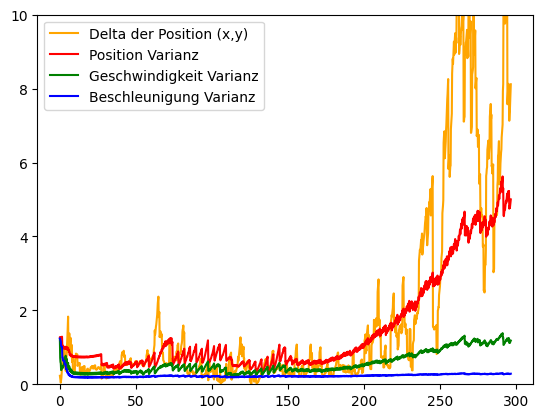
\includegraphics[width=.9\linewidth]{Ergebnisse/plots_ungenauigkeiten/winkel/winkel_const_vel_flag_freq.png}
        \caption{Zeitschritte 0-300}
    \end{subfigure}
    \begin{subfigure}{.5\textwidth}
        \centering
        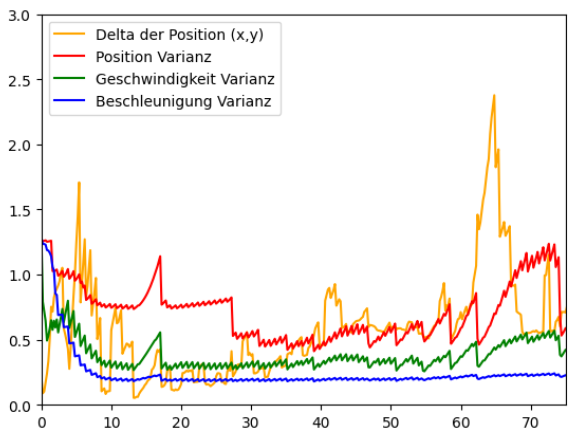
\includegraphics[width=.9\linewidth]{Ergebnisse/plots_ungenauigkeiten/winkel/winkel_ausschnitt.png}
        \caption{Zeitschritte 0-75}
        \label{subfig:varianz-closeup}
    \end{subfigure}
    \caption{Varianz beim Winkelansatz mit ausfallenden Türmen}
    \label{fig:varianz-visualisierung}
\end{figure*}




\subsection{Optimales Prozessrauschen}

% Ggfs. muss diese Beschreibung bereits in den Methoden-Teil!
Als wir zunächst die Filter unter denselben Filterbedingungen (insbesonders hinsichtlich des Prozessrauschens) vergleichen, deuteten die Ergebnisse schnell an, dass die verschiedenen Filter bei unterschiedlichen Filterbedingungen unterschiedlich gute Ergebnisse erzielten. Aus diesem Grund bestimmten wir grob einen optimalen Faktor für das Prozessrauschen (\(Q\)) für alle Filter. Die optimalen Faktoren sind gemeinsam mit ihrem korrespondierenden RMSE Wert in den Tabellen \ref{tab:optimal-Q-cv} und \ref{tab:optimal-Q-da} gelistet.

% Tabelle für optimales Q
\begin{table}[h]
\centering
\begin{tabular}{|l|c|c|c|}
\hline
\textbf{Filteransatz} & \textbf{Optimal} & \textbf{Var. Frequenz} & \textbf{Var. Freq. u. Ausfall} \\ \hline
Richtungen & 0.06, (0.39, 0.32)  & 0.01, (1.45, 1.22) & 0.01, (2.09, 1.15)   \\ \hline
Distanz & 0.01, (0.35, 0.39) & 0.01, (0.60, 0.83) & 0.01, (0.70, 1.02) \\ \hline
Winkel & 0.01, (0.41, 0.27) & 0.01, (2.28, 1.10) & 0.01, (2.27, 0.94) \\ \hline
\end{tabular}
\caption{Optimaler Q-Wert mit korrespondierenden RMSE-Werten (\(x\),\(y\)) bei konstanter Geschwindigkeit}
\label{tab:optimal-Q-cv}
\end{table}



% Tabelle für optimales Q
\begin{table}[h]
\centering
\begin{tabular}{|l|c|c|c|}
\hline
\textbf{Filteransatz} & \textbf{Optimal} & \textbf{Var. Frequenz} & \textbf{Var. Freq. u. Ausfall} \\ \hline
Richtungen & 6, (1.12, 0.65)  & 0.9, (2.05, 2.10) & 20, (6.19, 4.61)   \\ \hline
Distanz & 10, (0.47, 0.73) & 10, (1.34, 1.63) & 4, (1.38, 2.03) \\ \hline
Winkel & 9, (1.20, 0.76) & 3, (2.01, 2.12) & 10, (2.26, 2.31) \\ \hline
\end{tabular}
\caption{Optimaler Q-Wert mit korrespondierenden RMSE-Werten (\(x\),\(y\)) bei dynamischer Beschleunigung}
\label{tab:optimal-Q-da}
\end{table}



\section{Diskussion}

% \textbf{[SUNE HIER - mit Verweis auf alle Ergebnisse, Implikationen und Refs @ Anhang (gerne 1/2 -  3/4 Seite. Gerne auch Probleme+Lösungen die wir hatten]}


% TODO: Varianz - Frequenz-abhängigkeit Sägezahnmuster interpretieren
% TODO: Varianz - Ausfall beacon varianz-spike interpretieren



% ---

Die Forschungsfrage dieser Untersuchung lässt sich auf der Grundlage dieser Ergebnisse folgendermaßen beantworten.

Erwartungsgemäß erzielen alle Filter in Simulationsbedingungen mit besserer Messdatenlage stets bessere Ergebnisse (siehe Tabellen \ref{tab:cvRMSE} und \ref{tab:daRMSE}).

Senden Funktürme frequenz- oder ausfallbedingt nicht, so können, die Filter mithilfe ihrer Kovarianzmatrizen darauf reagieren, indem sie ihre eigenen Prognosen korrekterweise als weniger zuverlässig bewerteten (siehe beispielsweise die frequenzbedingte Sägezahnmuster in Abbildung \ref{fig:varianz-visualisierung} oder den Ausfall zwischen Zeitschritten 10 und 20 in Abbildung \ref{subfig:varianz-closeup}.
% Genauer werden? z.B: wie gut/wie schlecht schlägt sich welcher Filter bei verschiedenen Simulationsbedinungen?

Im Fall einer konstanten Geschwindigkeit erzielen alle Filter bei sehr geringem Prozessrauschen die besten Ergebnisse. Dies liegt in dem Umstand begründet, dass alle Filter ein constant-velocity Modell verwenden und ihre Vorhersagen entsprechenderweise so akkurat sind, dass sich die Filter weniger auf die verrauschten Messdaten verlassen müssen.
% Genauer werden? z.B: Haben unterschiedliche Filter hier unterschiedlich gut abgeschnitten

Bei dynamischer Beschleunigung ergeben sich für alle Filter individuelle, optimale Q-Faktoren für das Prozessrauschen. Dies lässt sich dadurch erklären, dass das constant-velocity-Modell der Filter bei dynamischen Beschleunigungen sehr fehleranfällig ist. Ein geringes Prozessrauschen führt in diesen Fällen dazu, dass der Filter seine Voraussagen im Vergleich zu den Messdaten zu positiv bewertet. Ein zu hohes Prozessrauschen resultiert darin, dass der Filter die (verrauschten) Messdaten im Verhältnis zu seinen eigenen Vorhersagen zu positiv bewertet, obwohl letztere weiterhin dazu in der Lage sind, trotz der fehlerhaften Beschleunigungsbeschreibung einigermaßen korrekte Vorhersagen zu treffen.
% Genauer werden? z.B: Q's näher beschreiben

Insgesamt lässt sich beobachten, dass der Richtungs- und Winkelansatz in Bezug auf die Orientierung eine bessere Leistung erzielt als der Entfernungsansatz (vergleiche hierzu beispielsweise die schlangenförmige Bewegung des Entfernungsansatzes mit den geraden Bewegungen des Richtungs- und Winkelansatzes in Abbildung \ref{fig:fahrtvisualisierung}).
Im Gegensatz dazu bestach der Entfernungsansatz bezüglich der Schätzung der zurückgelegten Distanz.

% Alles was auf Richtung/Winkel basiert, ist in Orientierung bessert (figure ...)
% Bei Entfernung ist Entfernung exakter



Die hier aufgeführten Ergebnisse sind ins Besondere im Kontext der folgenden beiden Limitationen zu verstehen. Zum einen entspricht im Richtungsfilter die vom Filter genutzte Standardabweichung der Messdaten nicht der Standardabweichung, welche beim Verrauschen der Messdaten verwendet wurde. % Näher ausführen?
Zum anderen ist es möglich, dass andere als die von uns verwendeten Filtereinstellung (ins Besonders im Bereich der Sigma-Punkte-Erzeugung, welche wir nicht gesondert betrachtet haben) zu anderen Ergebnissen führen können.

Betrachtet man die RMSE Werte der verschiedenen Filter-Ansätze, lässt sich feststellen, dass der Distanzansatz sowohl im direkten Vergleich bei identischen \(Q's\) (siehe Tabellen \ref{tab:cvRMSE} und \ref{tab:daRMSE}), als auch  unter Berücksichtigung des optimal gewählten Prozessrauschens (siehe Tabellen \ref{tab:optimal-Q-cv} und \ref{tab:optimal-Q-da}) die besten Ergebnisse liefert. 
Es sei an dieser Stelle jedoch angemerkt, dass die Bewertungsfunktion der verschiedenen Filteransätze prinzipiell nicht allein über den RMSE führen muss. Es könnte beispielsweise argumentiert werden, dass die Form der vorhergesagten Bewegung (siehe Abbildung \ref{fig:fahrtvisualisierung}) beim Entfernungsansatz am wenigsten der Originalbewegung ähnelt (siehe Abbildung \ref{fig:fahrtvisualisierung}). 




\begin{figure*}
    \begin{subfigure}{.333\textwidth}
        \centering
        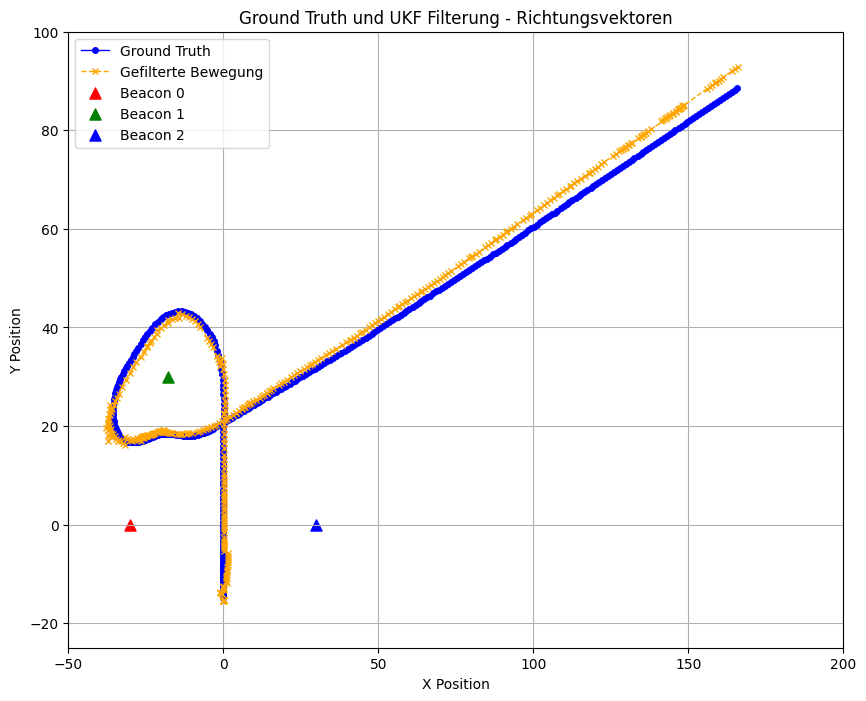
\includegraphics[width=.9\linewidth]{Ergebnisse/plots_fahrten/richtung/richtung_dyn_acc_flag_freq.png}
        \caption{Richtungsansatz}
    \end{subfigure}
    \begin{subfigure}{.333\textwidth}
        \centering
        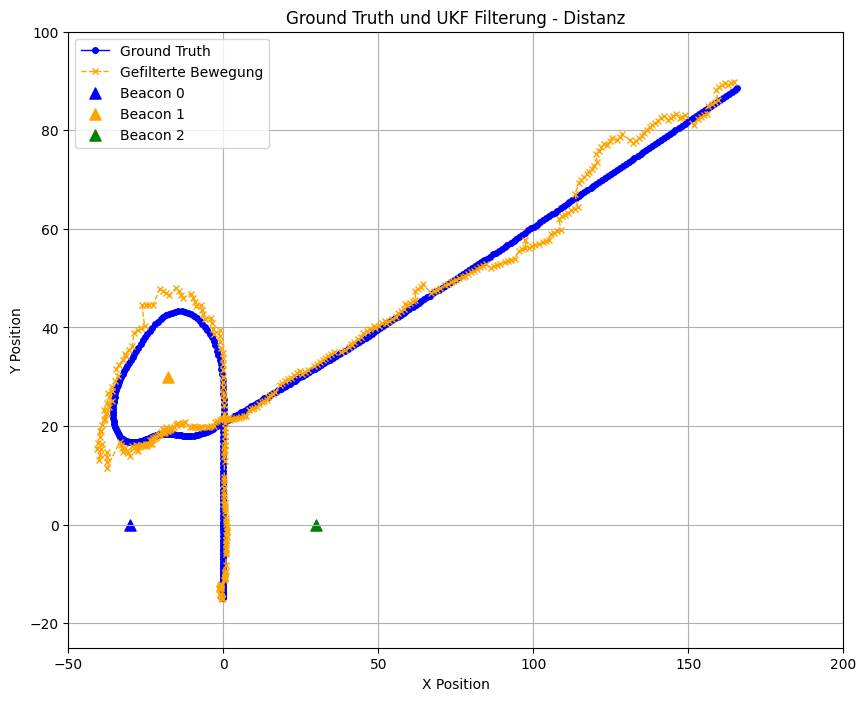
\includegraphics[width=.9\linewidth]{Ergebnisse/plots_fahrten/distanz/distanz_dyn_acc_flag_freq.png}
        \caption{Entfernungsansatz}
    \end{subfigure}
    \begin{subfigure}{.333\textwidth}
        \centering
        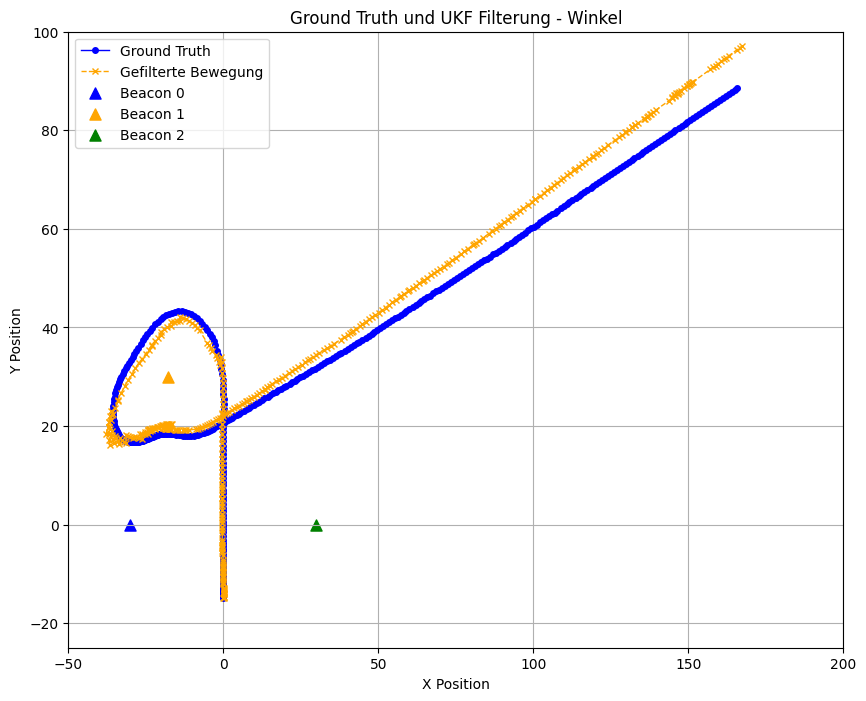
\includegraphics[width=.9\linewidth]{Ergebnisse/plots_fahrten/winkel/winkel_dyn_acc_flag_freq.png}
        \caption{Winkelansatz}
    \end{subfigure}
    \caption{Visualisierung Filterdaten bei unterschiedlich frequenten und ausfallenden Türmen}
    \label{fig:fahrtvisualisierung}
\end{figure*}




\section{Fazit}

Die hier ausgeführte Untersuchung beschäftigte sich mit dem Vergleich der Leistung von drei UKF-Implementationsansätzen bei unterschiedlichen Simulationsbedingungen. 

Zusammenfassend zeigen die Simulationsergebnisse, dass unter verbesserten Messdatenbedingungen alle Filter bessere Ergebnisse erzielen. Auf frequenzbedingte oder ausfallbedingte Datenausfälle reagieren alle Filter mithilfe ihrer Kovarianzmatrizen und bewerten ihre Prognosen als weniger zuverlässig.

Bei konstanter Geschwindigkeit liefern alle Filter bei geringem Prozessrauschen die besten Ergebnisse, da ihre Constant-Velocity Modelle genaue Vorhersagen ermöglichen und weniger auf verrauschte Messdaten angewiesen sind. Bei dynamischer Beschleunigung zeigen alle Filter unterschiedliche optimale Q-Faktoren für das Prozessrauschen, da das Constant-Velocity-Modell bei solchen Beschleunigungen fehleranfällig ist.

% Die Ergebnisse sind jedoch durch zwei Limitationen zu interpretieren: Die im Richtungsfilter verwendete Standardabweichung der Messdaten stimmt nicht mit der beim Verrauschen verwendeten Standardabweichung überein, und andere Filtereinstellungen könnten zu unterschiedlichen Ergebnissen führen, insbesondere im Bereich der Sigma-Punkte-Erzeugung.
Der Richtungsansatz besticht durch eine genaue Beschreibung der Orientierung und umgeht den Wrap-Around-Effekt. Jedoch entspricht die Standardabweichung in Grad nicht der verwendeten Standardabweichung in Metern. Mithilfe des Distanzansatzes lässt sich die Position sehr genau beschreiben und es tritt ebenfalls kein Wrap-Around-Effekt auf. Allerdings ist die Position erst ab drei sendenden Funktürmen eindeutig bestimmbar. Schließlich bringt der Winkelansatz eine genaue Beschreibung der Orientierung, leidet jedoch unter dem Wrap-Around Effekt, der sich aber im Verlauf der Implementation lösen ließ.

Die Bewertung der Filteransätze anhand der RMSE-Werte zeigt, dass der Distanzansatz die besten Ergebnisse liefert, sowohl im direkten Vergleich bei identischen Q-Faktoren als auch unter Berücksichtigung des optimalen Prozessrauschens. Es ist jedoch zu beachten, dass die Bewertungsfunktion nicht ausschließlich über den RMSE erfolgen sollte.



%\section{Danksagung}
%Die Autoren bedanken sich bei Prof. Dr. Torsten Edeler für die ausgezeichnete Vorlesung sowie seine stets verfügbare Unterstützung und hilfreichen Antworten bei aufkommenden Fragen. Seine Ratschläge während der Projektdurchführung waren für uns von großem Wert und haben maßgeblich zum Erfolg des Projekts beigetragen.

\subsection{Github}

Das Projekt ist unter der MIT-Lizenz frei verfügbar und kann unter dem folgenden Link eingesehen werden: \href{https://github.com/tkex/kalman-beacon}{https://github.com/tkex/kalman-beacon}

% Literatur
\bibliographystyle{IEEEtran}
\bibliography{lit}

% ---------------------------------------------------------

\newpage

% \label{sec:appendix}
% \section{Anhang}

% % Tabelle für konstante Geschwindigkeit
% \begin{table}[htbp]
% 	\centering
% 	\begin{tabular}{|l|c|c|c|}
% 		\hline
% 		\textbf{Filteransatz} & \textbf{Optimal} & \textbf{var. Frequenz} & \textbf{var. Freq. u. Ausfall} \\
% 		\hline
% 		Richtung & $0.9$ & $6.23$ & $6.64$ \\
% 		\hline
% 		Distanz & $0.8$ & $1.66$ & $1.88$\\
% 		\hline
% 		Winkel & $1.17$ & $5.18$ & $4.03$\\
% 		\hline
% 	\end{tabular}
% 	\caption{RMSE-Werte bei konstanter Geschwindigkeit (C.V.) mit ($Q*=0.1$)}
% 	\label{tab:rmse_constant_speed}
% \end{table}


% % Tabelle für dynamische Beschleunigung
% \begin{table}[htbp]
% 	\centering
% 	\begin{tabular}{|l|c|c|c|}
% 		\hline
% 		\textbf{Filteransatz} & \textbf{Optimal} & \textbf{Frequenz} & \textbf{Ausfall} \\
% 		\hline
% 		Richtung & $1.91$ & $4.13$ & $4.85$ \\
% 		\hline
% 		Distanz & $1.60$ & $3.73$ & $3.63$\\
% 		\hline
% 		Winkel & $2.31$ & $4.64$ & $7.11$\\
% 		\hline
% 	\end{tabular}
% 	\caption{RMSE-Werte bei dynamischer Beschleunigung (D.A.) mit $Q*=1$}
% 	\label{tab:rmse_dynamic_acceleration}
% \end{table}




% Beginn der Literaturliste
%\begin{thebibliography}{1}

%\bibitem{Labbe2024}
%R. Labbe, ``Kalman and Bayesian Filters in Python,'' 2024, [Online]. Verfügbar: \url{https://github.com/rlabbe/Kalman-and-Bayesian-Filters-in-Python}. [Zugriff am: 23. Februar 2024].


\newpage

\section{Anhang}

% ENTWEDER alle Ansätze mit einzelnen Plots visualisieren (2 x 3 er Figures)
% ODER:
%   Eine 3 x 3 er Figures für Fartvisualisierung 
%   und eine  3 x 3 er Figure für Fehler/Varianzen


% ------------------------- Ergebnisse: RICHTUNG -------------------------


% 3er-Figure Fahrtvisualisierung: Constant Velocity RICHTUNG 1) basic, 2) frequenz, 3) frequenz+ausfall
\begin{figure*}
    \begin{subfigure}{.333\textwidth}
        \centering
        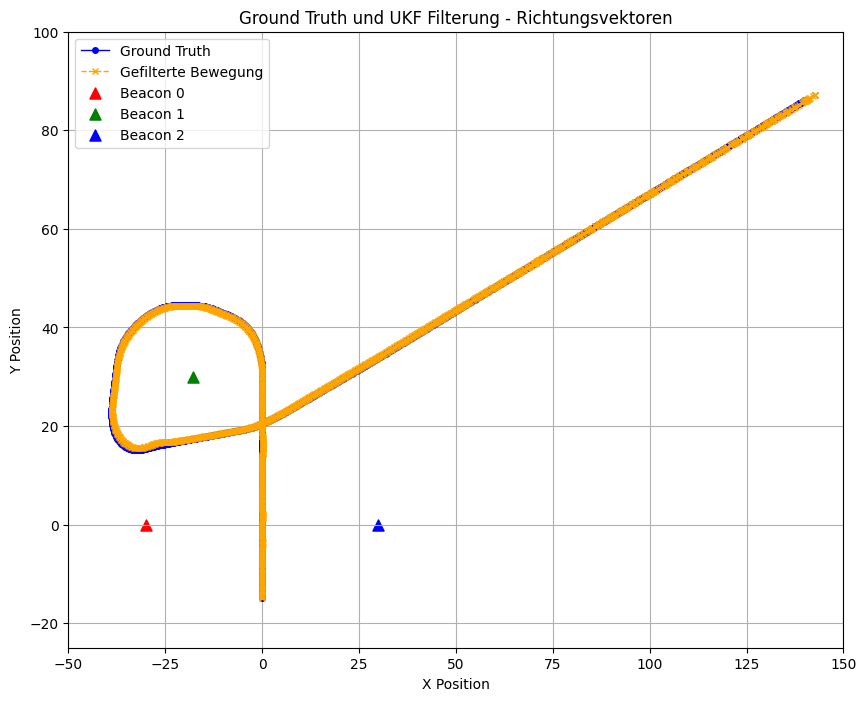
\includegraphics[width=.9\linewidth]{Ergebnisse/plots_fahrten/richtung/richtung_const_vel_basic.png}  
        \caption{Optimale Simulationsbedinungen}
        % \label{}
    \end{subfigure}    
    \begin{subfigure}{.333\textwidth}
        \centering
        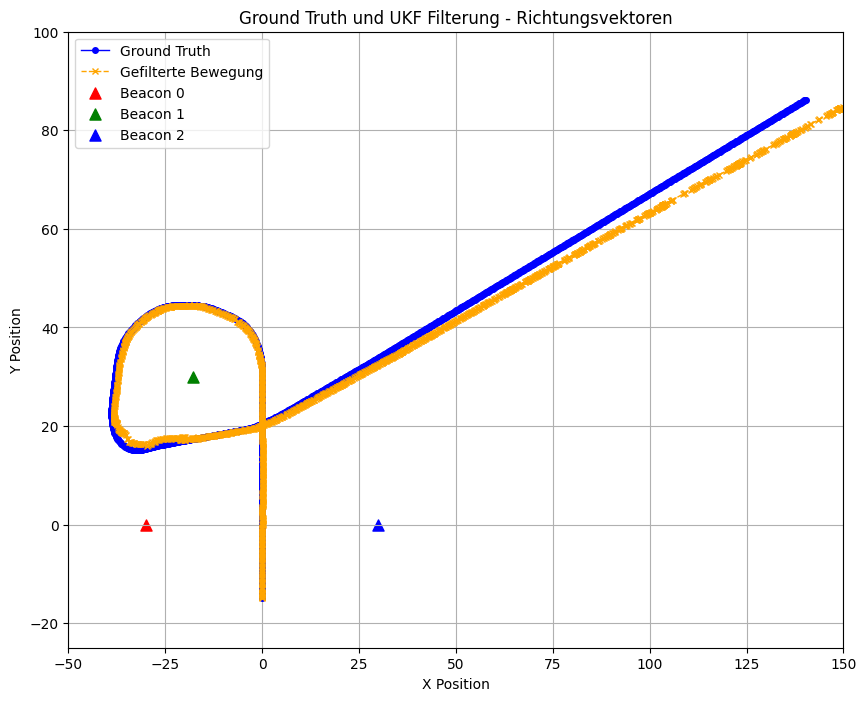
\includegraphics[width=.9\linewidth]{Ergebnisse/plots_fahrten/richtung/richtung_const_vel_freq.png} 
        \caption{Türme unterschiedlich frequent}
    \end{subfigure}    
    \begin{subfigure}{.333\textwidth}
        \centering
        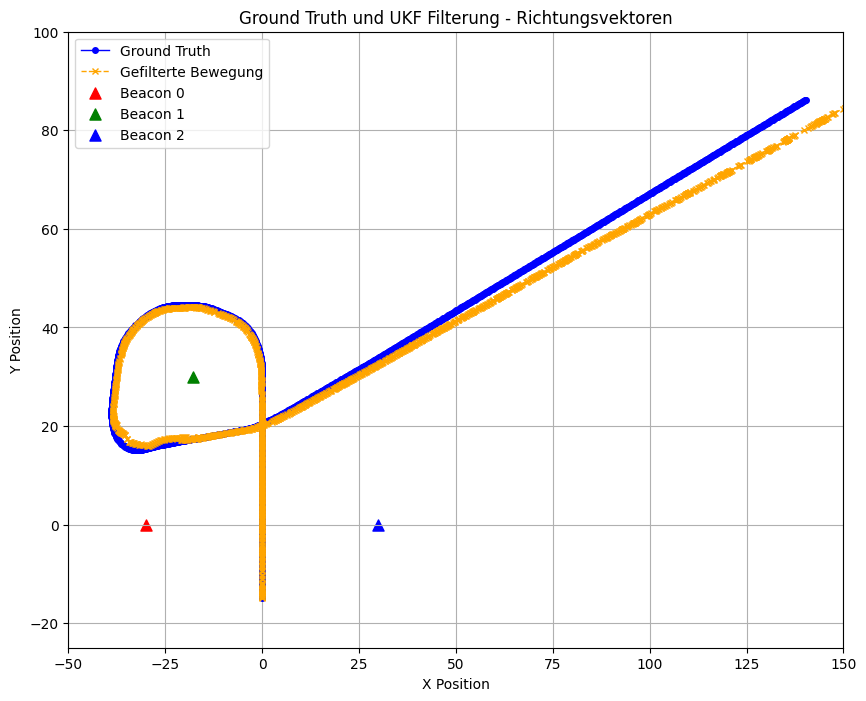
\includegraphics[width=.9\linewidth]{Ergebnisse/plots_fahrten/richtung/richtung_const_vel_flag_freq.png}
        \caption{Türme unterschiedlich frequent, ausfallend}
    \end{subfigure}
    \caption{Richtungsansatz: Ergebnisse bei konstanter Geschwindigkeit}
\end{figure*}


% 3er-Figure Fehler/Varianzen: Constant Velocity RICHTUNG 1) basic, 2) frequenz, 3) frequenz+ausfall
\begin{figure*}
    \begin{subfigure}{.333\textwidth}
        \centering
        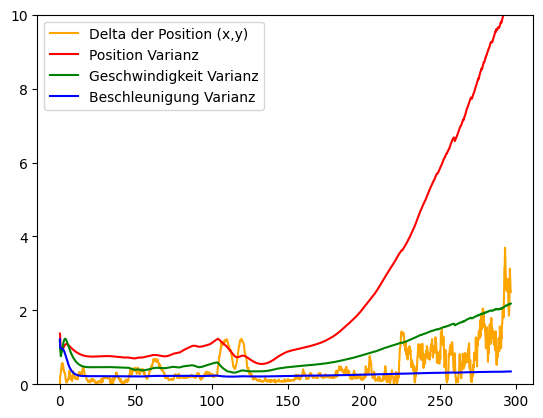
\includegraphics[width=.9\linewidth]{Ergebnisse/plots_ungenauigkeiten/richtung/richtung_const_vel_basic.png}
        \caption{Optimale Simulationsbedinungen}
    \end{subfigure}    
    \begin{subfigure}{.333\textwidth}
        \centering
        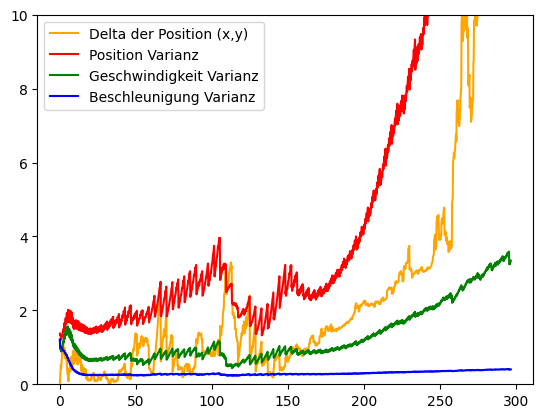
\includegraphics[width=.9\linewidth]{Ergebnisse/plots_ungenauigkeiten/richtung/richtung_const_vel_freq.png}
        \caption{Türme unterschiedlich frequent}
    \end{subfigure}    
    \begin{subfigure}{.333\textwidth}
        \centering
        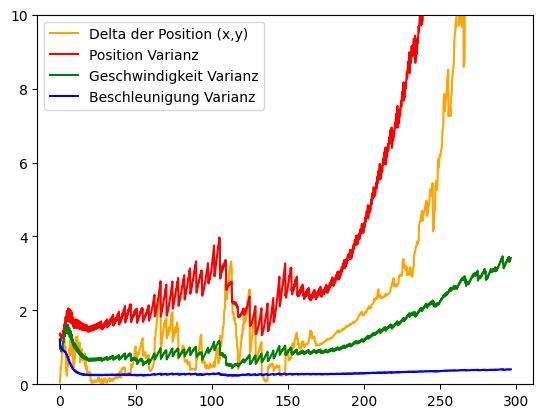
\includegraphics[width=.9\linewidth]{Ergebnisse/plots_ungenauigkeiten/richtung/richtung_const_vel_flag_freq.png}
        \caption{Türme unterschiedlich frequent, ausfallend}
    \end{subfigure}
    \caption{Richtungsansatz: Fehler und Varianzen bei konstanter Geschwindigkeit}
    \label{abb:richtung-cv-fehler}
\end{figure*}




% % ------------------------- Ergebnisse: ENTFERNUNG -------------------------

% \subsubsection{Entfernungsansatz}

% 3er-Figure Fahrtvisualisierung: Constant Velocity ENTFERNUNG 1) basic, 2) frequenz, 3) frequenz+ausfall
\begin{figure*}
    \begin{subfigure}{.333\textwidth}
        \centering
        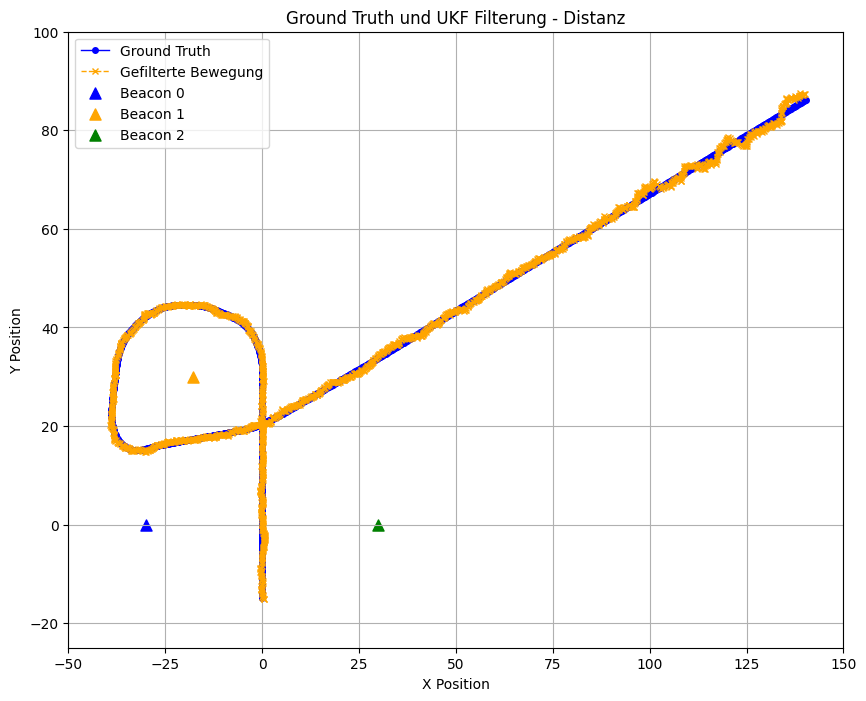
\includegraphics[width=.9\linewidth]{Ergebnisse/plots_fahrten/distanz/distanz_const_vel_basic.png}  
        \caption{Optimale Simulationsbedinungen}
    \end{subfigure}    
    \begin{subfigure}{.333\textwidth}
        \centering
        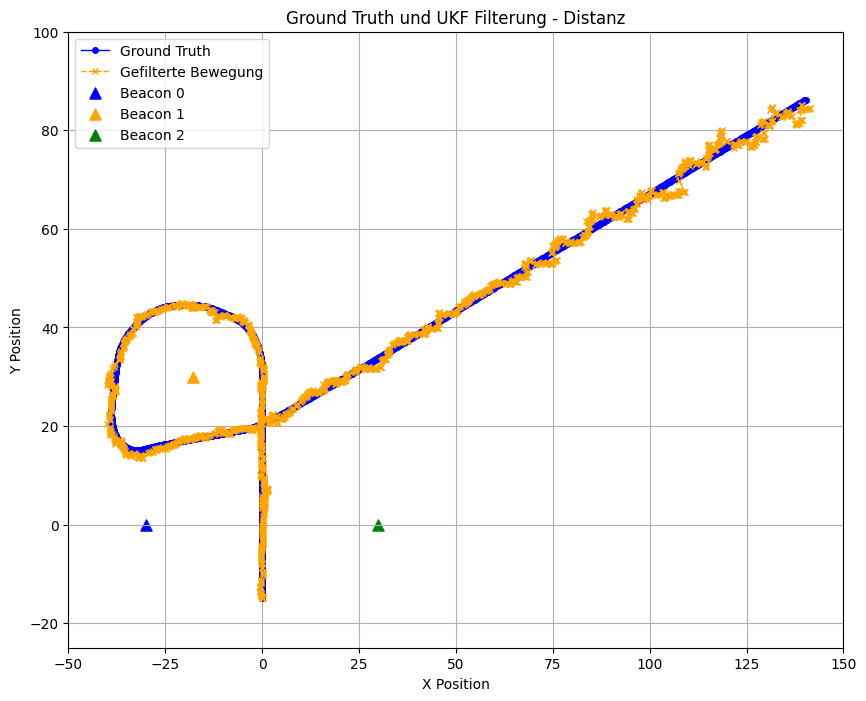
\includegraphics[width=.9\linewidth]{Ergebnisse/plots_fahrten/distanz/distanz_const_vel_freq.png} 
        \caption{Türme unterschiedlich frequent}
    \end{subfigure}    
    \begin{subfigure}{.333\textwidth}
        \centering
        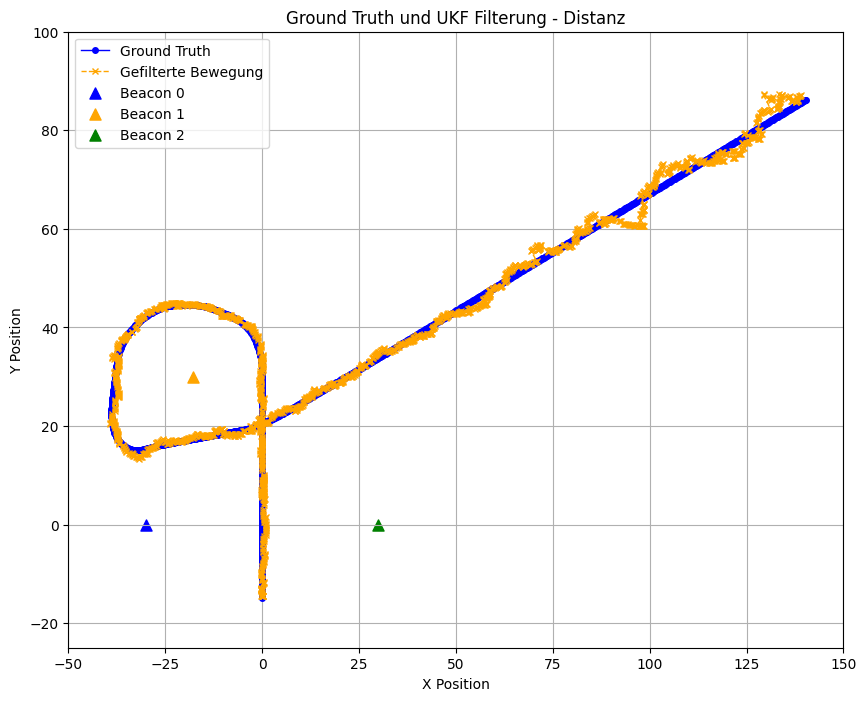
\includegraphics[width=.9\linewidth]{Ergebnisse/plots_fahrten/distanz/distanz_const_vel_flag_freq.png}
        \caption{Türme unterschiedlich frequent, ausfallend}
    \end{subfigure}
    \caption{Entfernungsansatz: Ergebnisse bei konstanter Geschwindigkeit}
\end{figure*}


% 3er-Figure Fahrtvisualisierung: Constant Velocity ENTFERNUNG 1) basic, 2) frequenz, 3) frequenz+ausfall
\begin{figure*}
    \begin{subfigure}{.333\textwidth}
        \centering
        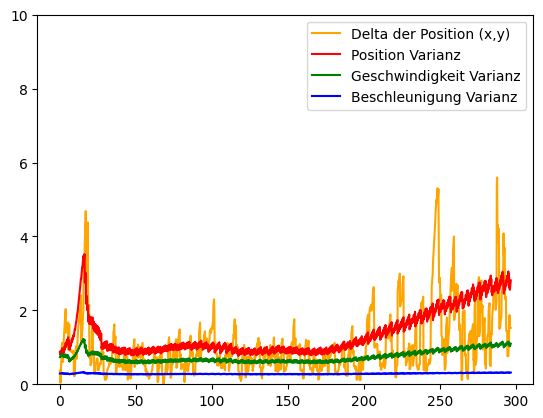
\includegraphics[width=.9\linewidth]{Ergebnisse/plots_ungenauigkeiten/distanz/distanz_const_vel_flag_freq.png}
        \caption{Optimale Simulationsbedinungen}
    \end{subfigure}    
    \begin{subfigure}{.333\textwidth}
        \centering
        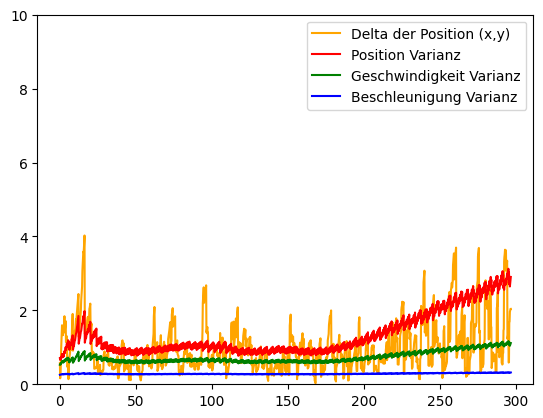
\includegraphics[width=.9\linewidth]{Ergebnisse/plots_ungenauigkeiten/distanz/distanz_const_vel_freq.png}
        \caption{Türme unterschiedlich frequent}
    \end{subfigure}    
    \begin{subfigure}{.333\textwidth}
        \centering
        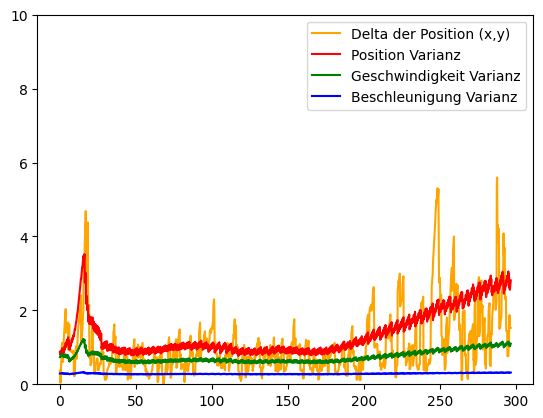
\includegraphics[width=.9\linewidth]{Ergebnisse/plots_ungenauigkeiten/distanz/distanz_const_vel_flag_freq.png}
        \caption{Türme unterschiedlich frequent, ausfallend}
    \end{subfigure}
    \label{abb:distanz-cv-fehler}
    \caption{Entfernungsansatz: Fehler und Varianzen bei konstanter Geschwindigkeit}
\end{figure*}




% % ------------------------- Ergebnisse: WINKEL -------------------------

% \subsubsection{Winkelansatz}

% 3er-Figure Fahrtvisualisierung: Constant Velocity WINKEL 1) basic, 2) frequenz, 3) frequenz+ausfall
\begin{figure*}
    \begin{subfigure}{.333\textwidth}
        \centering
        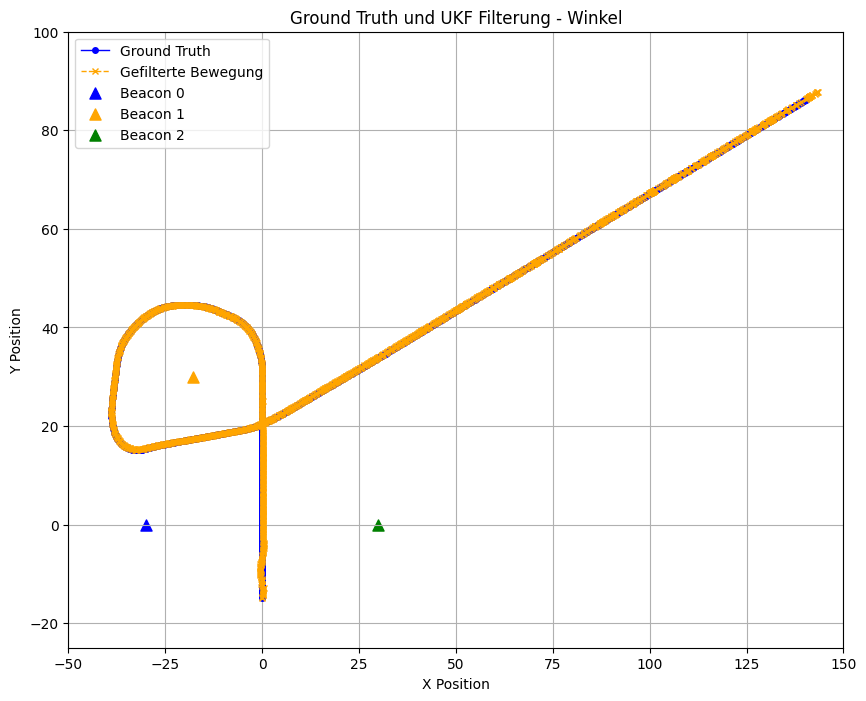
\includegraphics[width=.9\linewidth]{Ergebnisse/plots_fahrten/winkel/winkel_const_vel_basic.png}  
        \caption{Optimale Simulationsbedinungen}
        % \label{}
    \end{subfigure}    
    \begin{subfigure}{.333\textwidth}
        \centering
        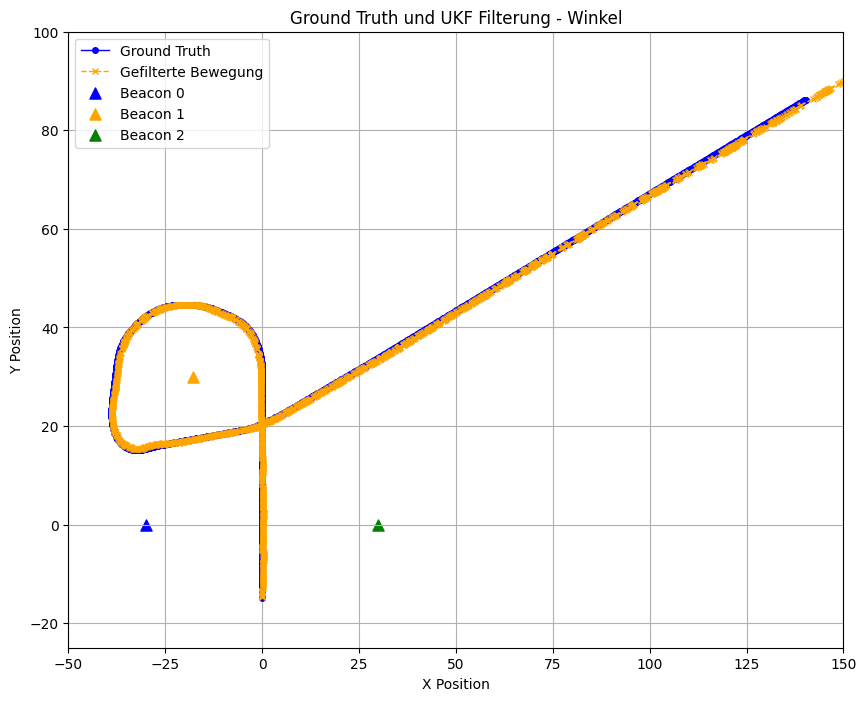
\includegraphics[width=.9\linewidth]{Ergebnisse/plots_fahrten/winkel/winkel_const_vel_freq.png} 
        \caption{Türme unterschiedlich frequent}
    \end{subfigure}    
    \begin{subfigure}{.333\textwidth}
        \centering
        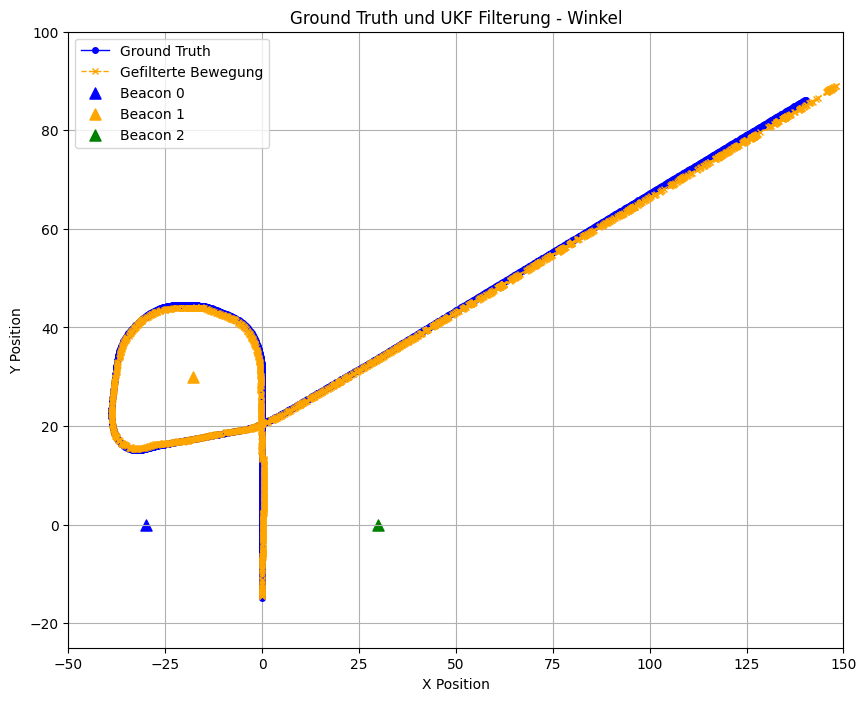
\includegraphics[width=.9\linewidth]{Ergebnisse/plots_fahrten/winkel/winkel_const_vel_flag_freq.png}
        \caption{Türme unterschiedlich frequent, ausfallend}
    \end{subfigure}
    \caption{Winkelansatz: Ergebnisse bei konstanter Geschwindigkeit}
\end{figure*}

% 3er-Figure Fehler/Varianzen: Constant Velocity WINKEL 1) basic, 2) frequenz, 3) frequenz+ausfall
\begin{figure*}
    \begin{subfigure}{.333\textwidth}
        \centering
        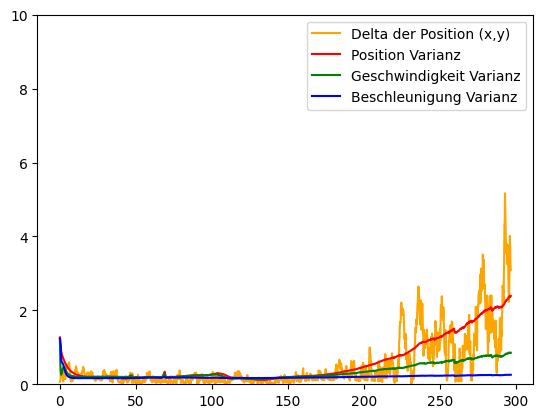
\includegraphics[width=.9\linewidth]{Ergebnisse/plots_ungenauigkeiten/winkel/winkel_const_vel_basic.png}  
        \caption{Optimale Simulationsbedinungen}
        % \label{}
    \end{subfigure}    
    \begin{subfigure}{.333\textwidth}
        \centering
        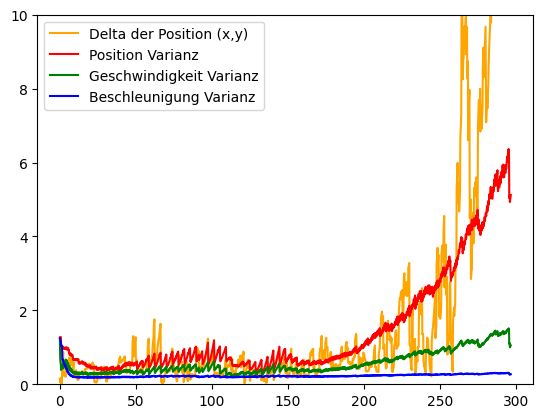
\includegraphics[width=.9\linewidth]{Ergebnisse/plots_ungenauigkeiten/winkel/winkel_const_vel_freq.png}  
        \caption{Türme unterschiedlich frequent}
    \end{subfigure}    
    \begin{subfigure}{.333\textwidth}
        \centering
        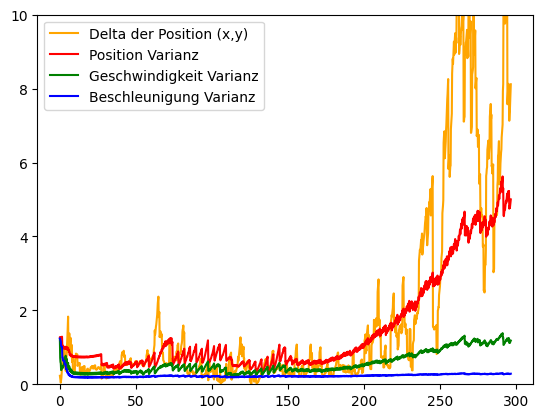
\includegraphics[width=.9\linewidth]{Ergebnisse/plots_ungenauigkeiten/winkel/winkel_const_vel_flag_freq.png}
        \caption{Türme unterschiedlich frequent, ausfallend}
    \end{subfigure}
    \caption{Winkelansatz: Fehler und Varianzen bei konstanter Geschwindigkeit}
    \label{abb:winkel-cv-fehler}
\end{figure*}



% im Vergleich lässt sich sagen, dass ... unter den in Figur ... dargestellten Filtereinstellungen am besten abschneidet.
% Wird Q optimal gesetzt, kann ... einen RMSE von bis zu ... erreichen. (Entweder besser oder schlechter als was auch immer unter nicht-Q-optimierten Bedingungen "gewonnen" hat)

% \subsection{Dynamische Geschwindigkeit}

%  ------------------------- Ergebnisse: RICHTUNG -------------------------

% \subsubsection{Richtungsansatz}

% 3er-Figure Fahrtvisualisierung: Dynamic Acceleration RICHTUNG 1) basic, 2) frequenz, 3) frequenz+ausfall
\begin{figure*}
    \begin{subfigure}{.333\textwidth}
        \centering
        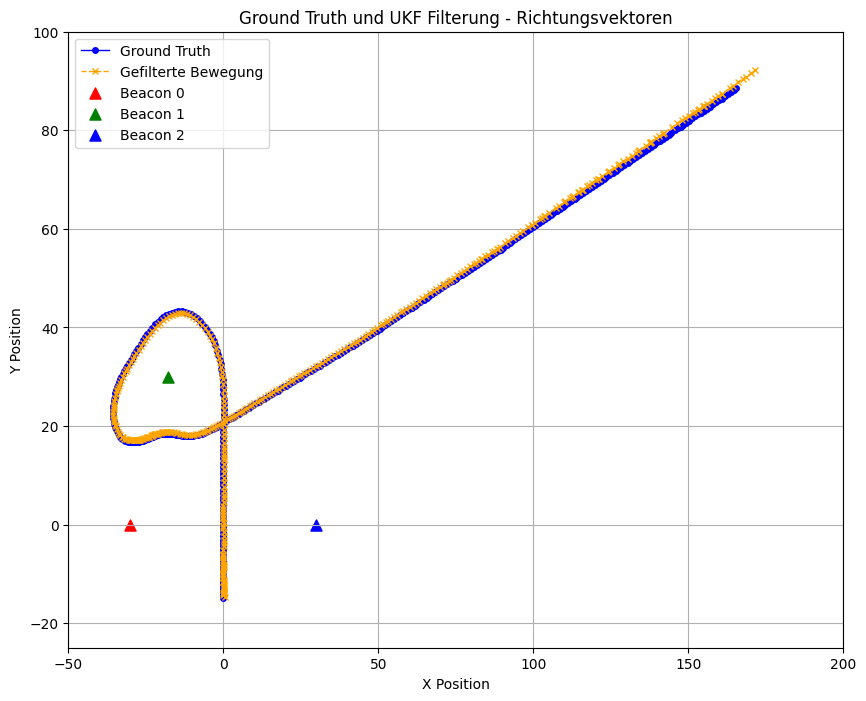
\includegraphics[width=.9\linewidth]{Ergebnisse/plots_fahrten/richtung/richtung_dyn_acc_basic.png}  
        \caption{Optimale Simulationsbedinungen}
        % \label{}
    \end{subfigure}    
    \begin{subfigure}{.333\textwidth}
        \centering
        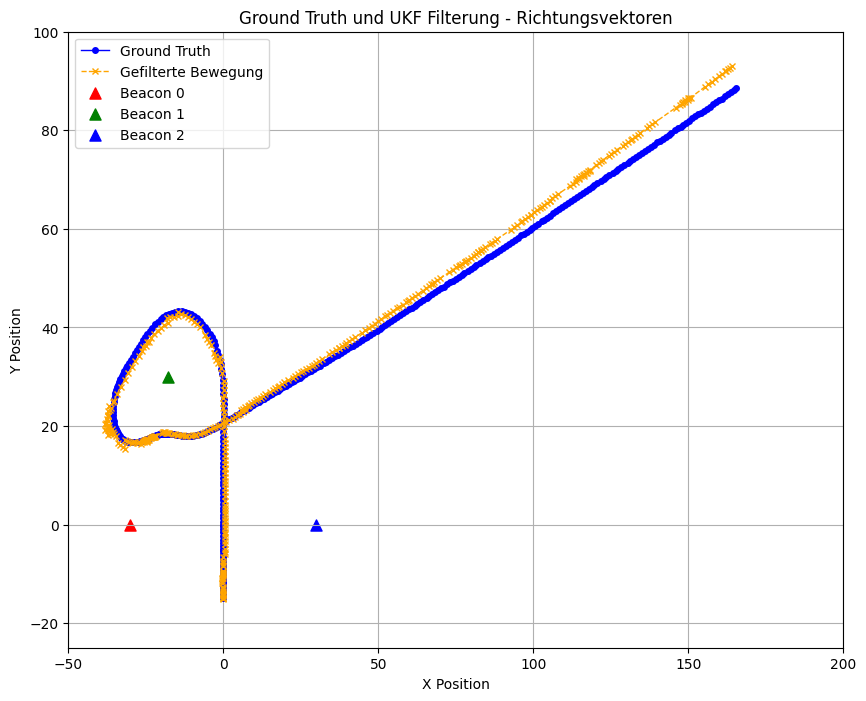
\includegraphics[width=.9\linewidth]{Ergebnisse/plots_fahrten/richtung/richtung_dyn_acc_freq.png} 
        \caption{Türme unterschiedlich frequent}
    \end{subfigure}    
    \begin{subfigure}{.333\textwidth}
        \centering
        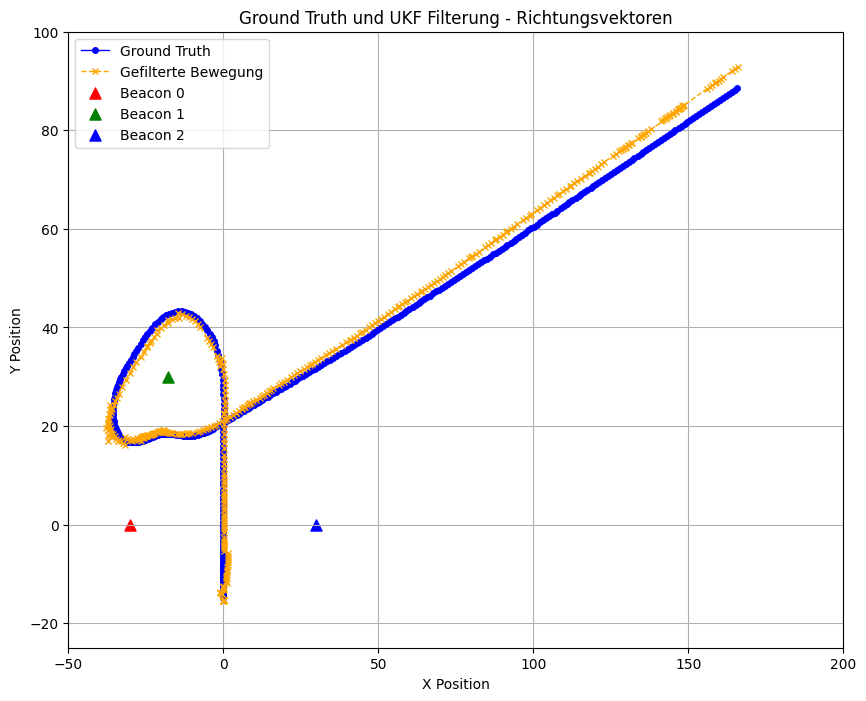
\includegraphics[width=.9\linewidth]{Ergebnisse/plots_fahrten/richtung/richtung_dyn_acc_flag_freq.png}
        \caption{Türme unterschiedlich frequent, ausfallend}
    \end{subfigure}
    \caption{Richtungsansatz: Ergebnisse bei konstanter Geschwindigkeit}
\end{figure*}

% 3er-Figure Fehler/Varianzen: Dynamic Acceleration RICHTUNG 1) basic, 2) frequenz, 3) frequenz+ausfall
\begin{figure*}
    \begin{subfigure}{.333\textwidth}
        \centering
        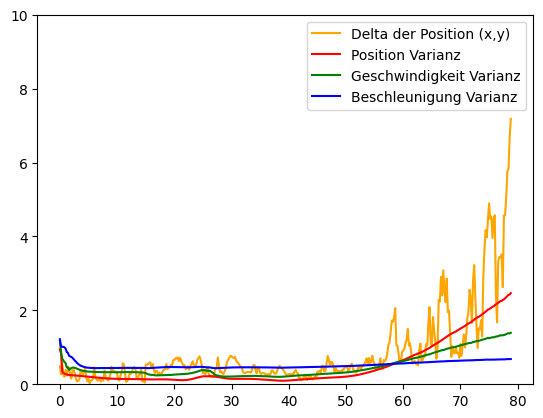
\includegraphics[width=.9\linewidth]{Ergebnisse/plots_ungenauigkeiten/richtung/richtung_dyn_acc_basic.png}
        \caption{Optimale Simulationsbedinungen}
    \end{subfigure}    
    \begin{subfigure}{.333\textwidth}
        \centering
        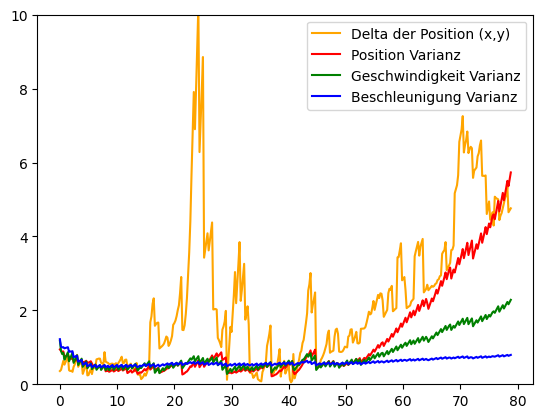
\includegraphics[width=.9\linewidth]{Ergebnisse/plots_ungenauigkeiten/richtung/richtung_dyn_acc_freq.png}
        \caption{Türme unterschiedlich frequent}
    \end{subfigure}    
    \begin{subfigure}{.333\textwidth}
        \centering
        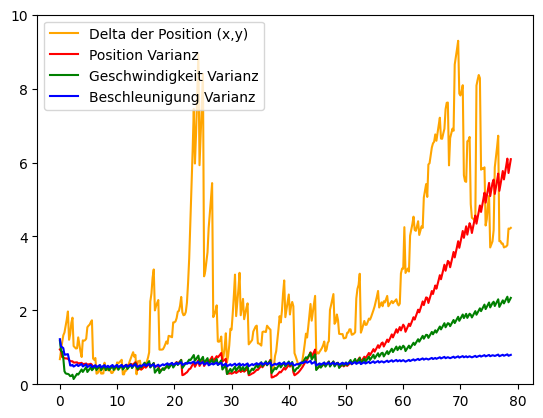
\includegraphics[width=.9\linewidth]{Ergebnisse/plots_ungenauigkeiten/richtung/richtung_dyn_acc_flag_freq.png}
        \caption{Türme unterschiedlich frequent, ausfallend}
    \end{subfigure}
    \caption{Richtungsansatz: Fehler und Varianzen bei konstanter Geschwindigkeit}
    \label{abb:richtung-da-fehler}
\end{figure*}


% % ------------------------- Ergebnisse: ENTFERNUNG -------------------------

% \subsubsection{Entfernungsansatz}

% 3er-Figure Fahrtvisualisierung: Dynamic Acceleration ENTFERNUNG 1) basic, 2) frequenz, 3) frequenz+ausfall
\begin{figure*}
    \begin{subfigure}{.333\textwidth}
        \centering
        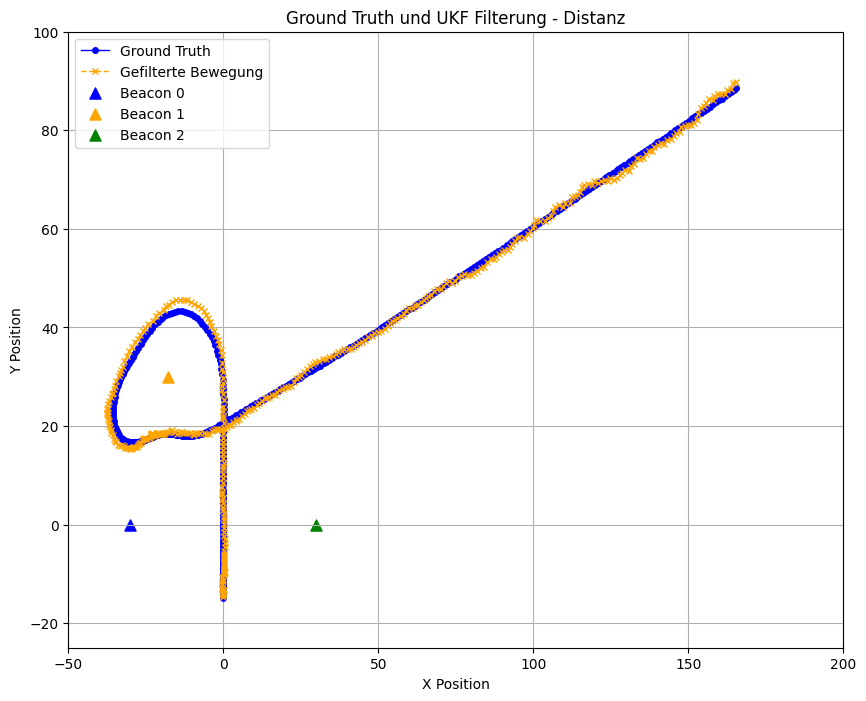
\includegraphics[width=.9\linewidth]{Ergebnisse/plots_fahrten/distanz/distanz_dyn_acc_basic.png}  
        \caption{Optimale Simulationsbedinungen}
    \end{subfigure}    
    \begin{subfigure}{.333\textwidth}
        \centering
        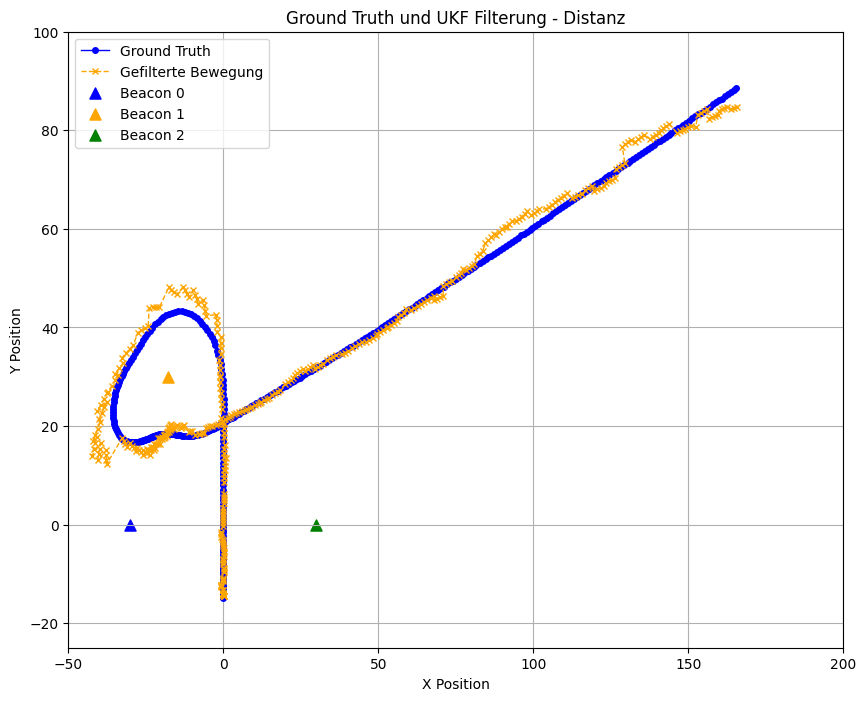
\includegraphics[width=.9\linewidth]{Ergebnisse/plots_fahrten/distanz/distanz_dyn_acc_freq.png} 
        \caption{Türme unterschiedlich frequent}
    \end{subfigure}    
    \begin{subfigure}{.333\textwidth}
        \centering
        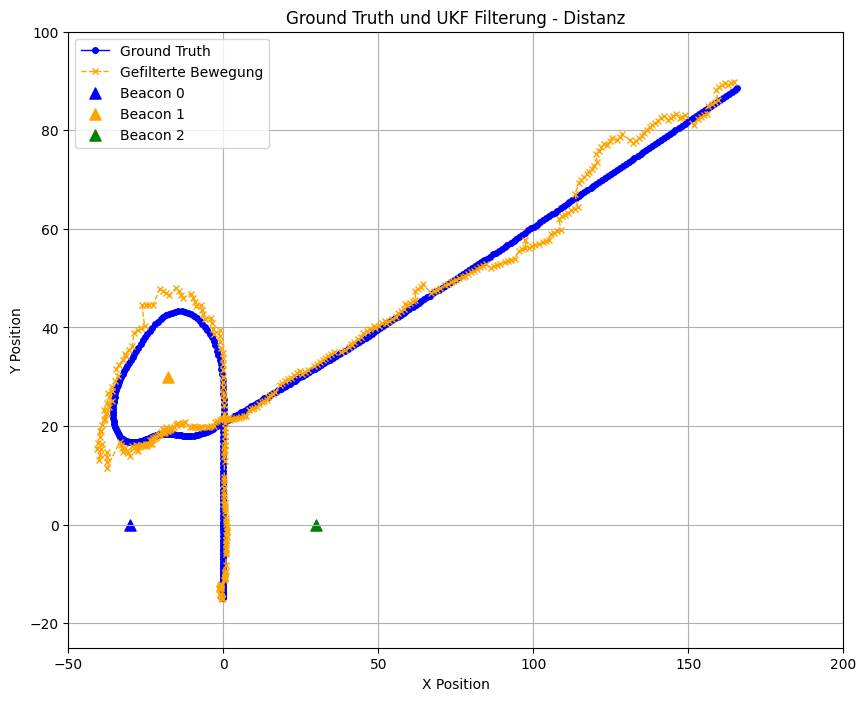
\includegraphics[width=.9\linewidth]{Ergebnisse/plots_fahrten/distanz/distanz_dyn_acc_flag_freq.png}
        \caption{Türme unterschiedlich frequent, ausfallend}
    \end{subfigure}
    \caption{Entfernungsansatz: Ergebnisse bei konstanter Geschwindigkeit}
\end{figure*}


% 3er-Figure Fahrtvisualisierung: Dynamic Acceleration ENTFERNUNG 1) basic, 2) frequenz, 3) frequenz+ausfall
\begin{figure*}
    \begin{subfigure}{.333\textwidth}
        \centering
        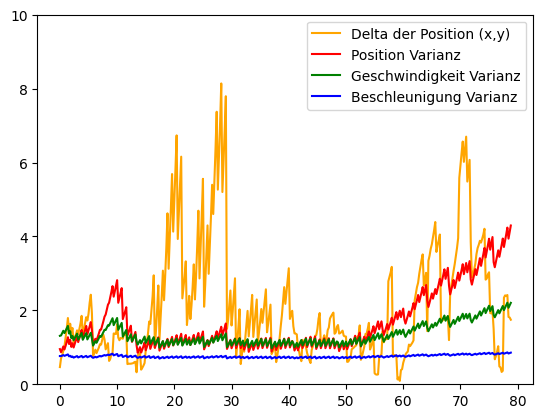
\includegraphics[width=.9\linewidth]{Ergebnisse/plots_ungenauigkeiten/distanz/distanz_dyn_acc_flag_freq.png}
        \caption{Optimale Simulationsbedinungen}
    \end{subfigure}    
    \begin{subfigure}{.333\textwidth}
        \centering
        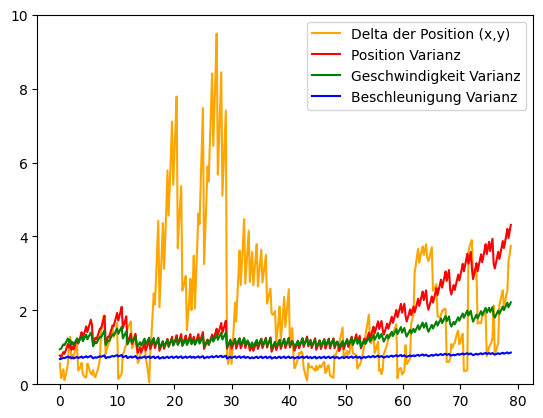
\includegraphics[width=.9\linewidth]{Ergebnisse/plots_ungenauigkeiten/distanz/distanz_dyn_acc_freq.png}
        \caption{Türme unterschiedlich frequent}
    \end{subfigure}    
    \begin{subfigure}{.333\textwidth}
        \centering
        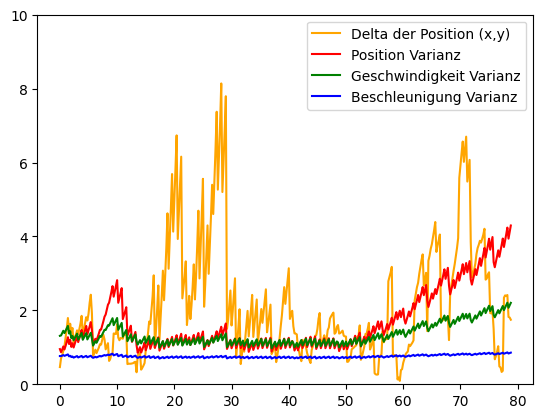
\includegraphics[width=.9\linewidth]{Ergebnisse/plots_ungenauigkeiten/distanz/distanz_dyn_acc_flag_freq.png}
        \caption{Türme unterschiedlich frequent, ausfallend}
    \end{subfigure}
    \caption{Entfernungsansatz: Fehler und Varianzen bei konstanter Geschwindigkeit}
    \label{abb:distanz-da-fehler}
\end{figure*}



% % ------------------------- Ergebnisse: WINKEL -------------------------

% \subsubsection{Winkelansatz}

% 3er-Figure Fahrtvisualisierung: Dynamic Acceleration WINKEL 1) basic, 2) frequenz, 3) frequenz+ausfall
\begin{figure*}
    \begin{subfigure}{.333\textwidth}
        \centering
        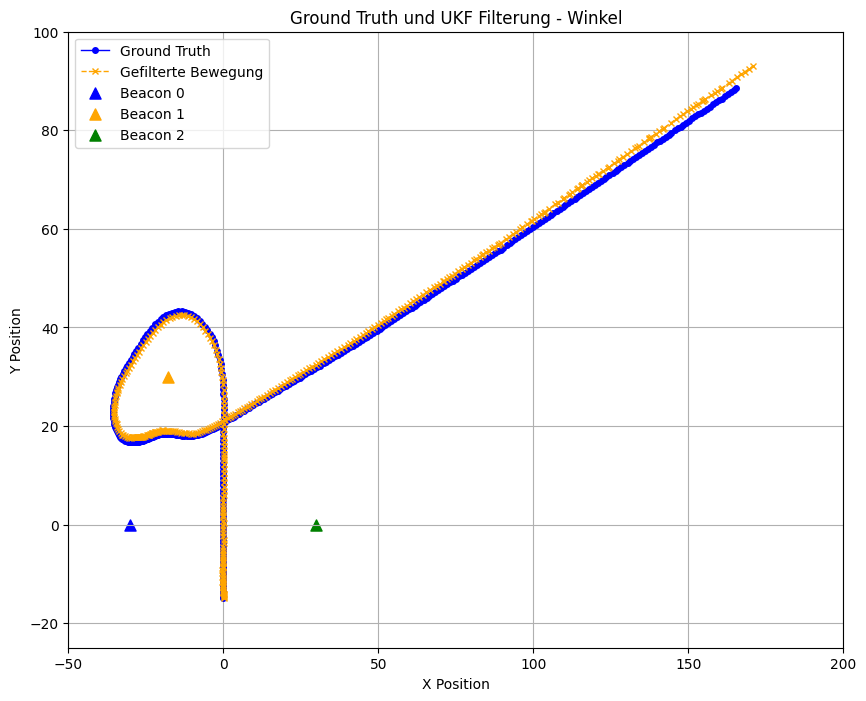
\includegraphics[width=.9\linewidth]{Ergebnisse/plots_fahrten/winkel/winkel_dyn_acc_basic.png}  
        \caption{Optimale Simulationsbedinungen}
        % \label{}
    \end{subfigure}    
    \begin{subfigure}{.333\textwidth}
        \centering
        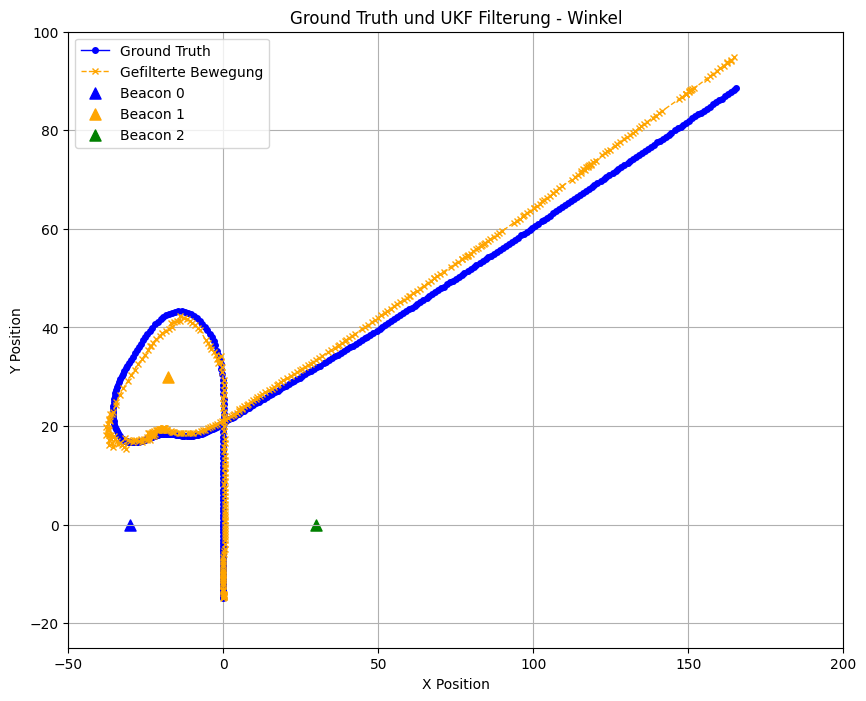
\includegraphics[width=.9\linewidth]{Ergebnisse/plots_fahrten/winkel/winkel_dyn_acc_freq.png} 
        \caption{Türme unterschiedlich frequent}
    \end{subfigure}    
    \begin{subfigure}{.333\textwidth}
        \centering
        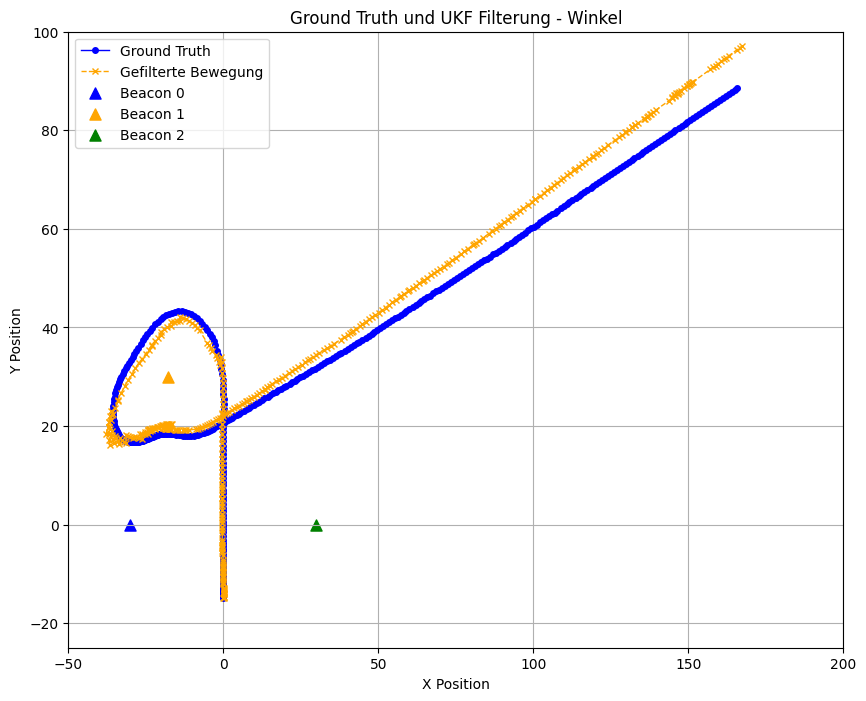
\includegraphics[width=.9\linewidth]{Ergebnisse/plots_fahrten/winkel/winkel_dyn_acc_flag_freq.png}
        \caption{Türme unterschiedlich frequent, ausfallend}
    \end{subfigure}
    \caption{Winkelansatz: Ergebnisse bei konstanter Geschwindigkeit}
\end{figure*}

% 3er-Figure Fehler/Varianzen: Dynamic Acceleration WINKEL 1) basic, 2) frequenz, 3) frequenz+ausfall
\begin{figure*}
    \begin{subfigure}{.333\textwidth}
        \centering
        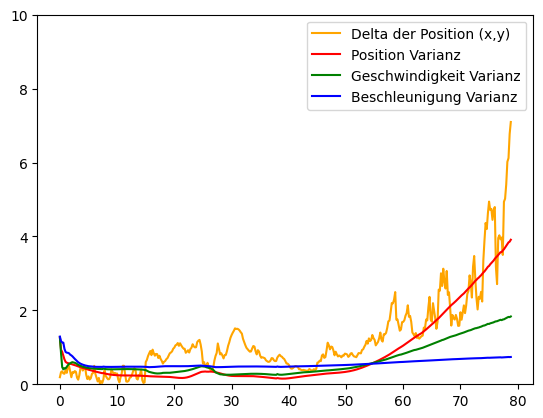
\includegraphics[width=.9\linewidth]{Ergebnisse/plots_ungenauigkeiten/winkel/winkel_dyn_acc_basic.png}  
        \caption{Optimale Simulationsbedinungen}
        % \label{}
    \end{subfigure}    
    \begin{subfigure}{.333\textwidth}
        \centering
        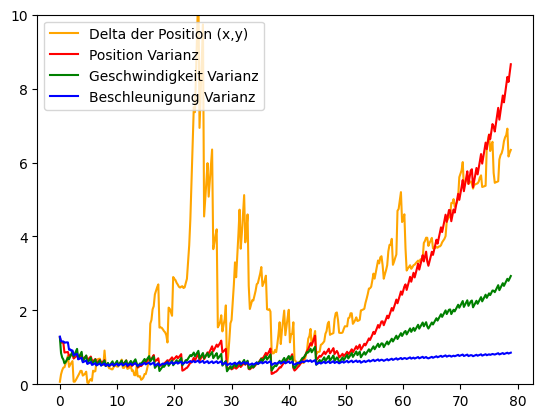
\includegraphics[width=.9\linewidth]{Ergebnisse/plots_ungenauigkeiten/winkel/winkel_dyn_acc_freq.png}  
        \caption{Türme unterschiedlich frequent}
    \end{subfigure}    
    \begin{subfigure}{.333\textwidth}
        \centering
        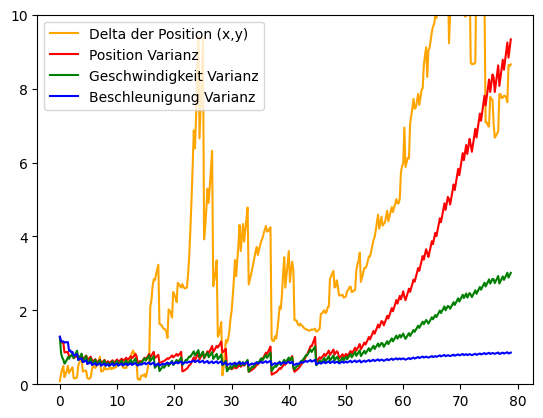
\includegraphics[width=.9\linewidth]{Ergebnisse/plots_ungenauigkeiten/winkel/winkel_dyn_acc_flag_freq.png}
        \caption{Türme unterschiedlich frequent, ausfallend}
    \end{subfigure}
    \caption{Winkelansatz: Fehler und Varianzen bei konstanter Geschwindigkeit}
    \label{abb:winkel-da-fehler}
\end{figure*}

% im Vergleich lässt sich sagen, dass ... bei optimalen Bedingungen am besten abschneidet




\end{document}
